\documentclass[11pt,letterpaper]{article}

\usepackage{color}
\usepackage{graphicx}
\usepackage{adjustbox}
\usepackage{subcaption}
\usepackage{float}
\usepackage{chngpage}
\usepackage{enumerate}
\usepackage{boxedminipage}
\usepackage{bold-extra}
\usepackage{cite}
\usepackage{gensymb}
\usepackage{array}
\usepackage{longtable}
\usepackage{amsmath}
\usepackage{times} %change font to Times
\usepackage[left=1.25in,right=1.25in,top=1.25in,bottom=1.25in]{geometry}
\usepackage{setspace} %Enables some environments to change spacing
\usepackage{titlesec,titletoc} %Enables title and section formatting
\usepackage{booktabs} %Fancy rules for tables
\usepackage[font={small}]{caption} %Reduces font-size for captions
\usepackage{lineno} %Enables line numbers
%\linenumbers %Put line numbers. Comment to have the final version
\usepackage{appendix}
\usepackage{listings}
\usepackage{multicol}
\usepackage{wrapfig}
\usepackage[section]{placeins}

%Format the line spacing
\linespread{1.3} %1.3=one and a half, 1.6=2
\setlength\parindent{0.5in}


\title{Capstone 1:\\Fossil fuel economies in the United States}
\author{Rahul Verma}

\begin{document}
\graphicspath{{./Images/}}
\maketitle

\begin{figure}
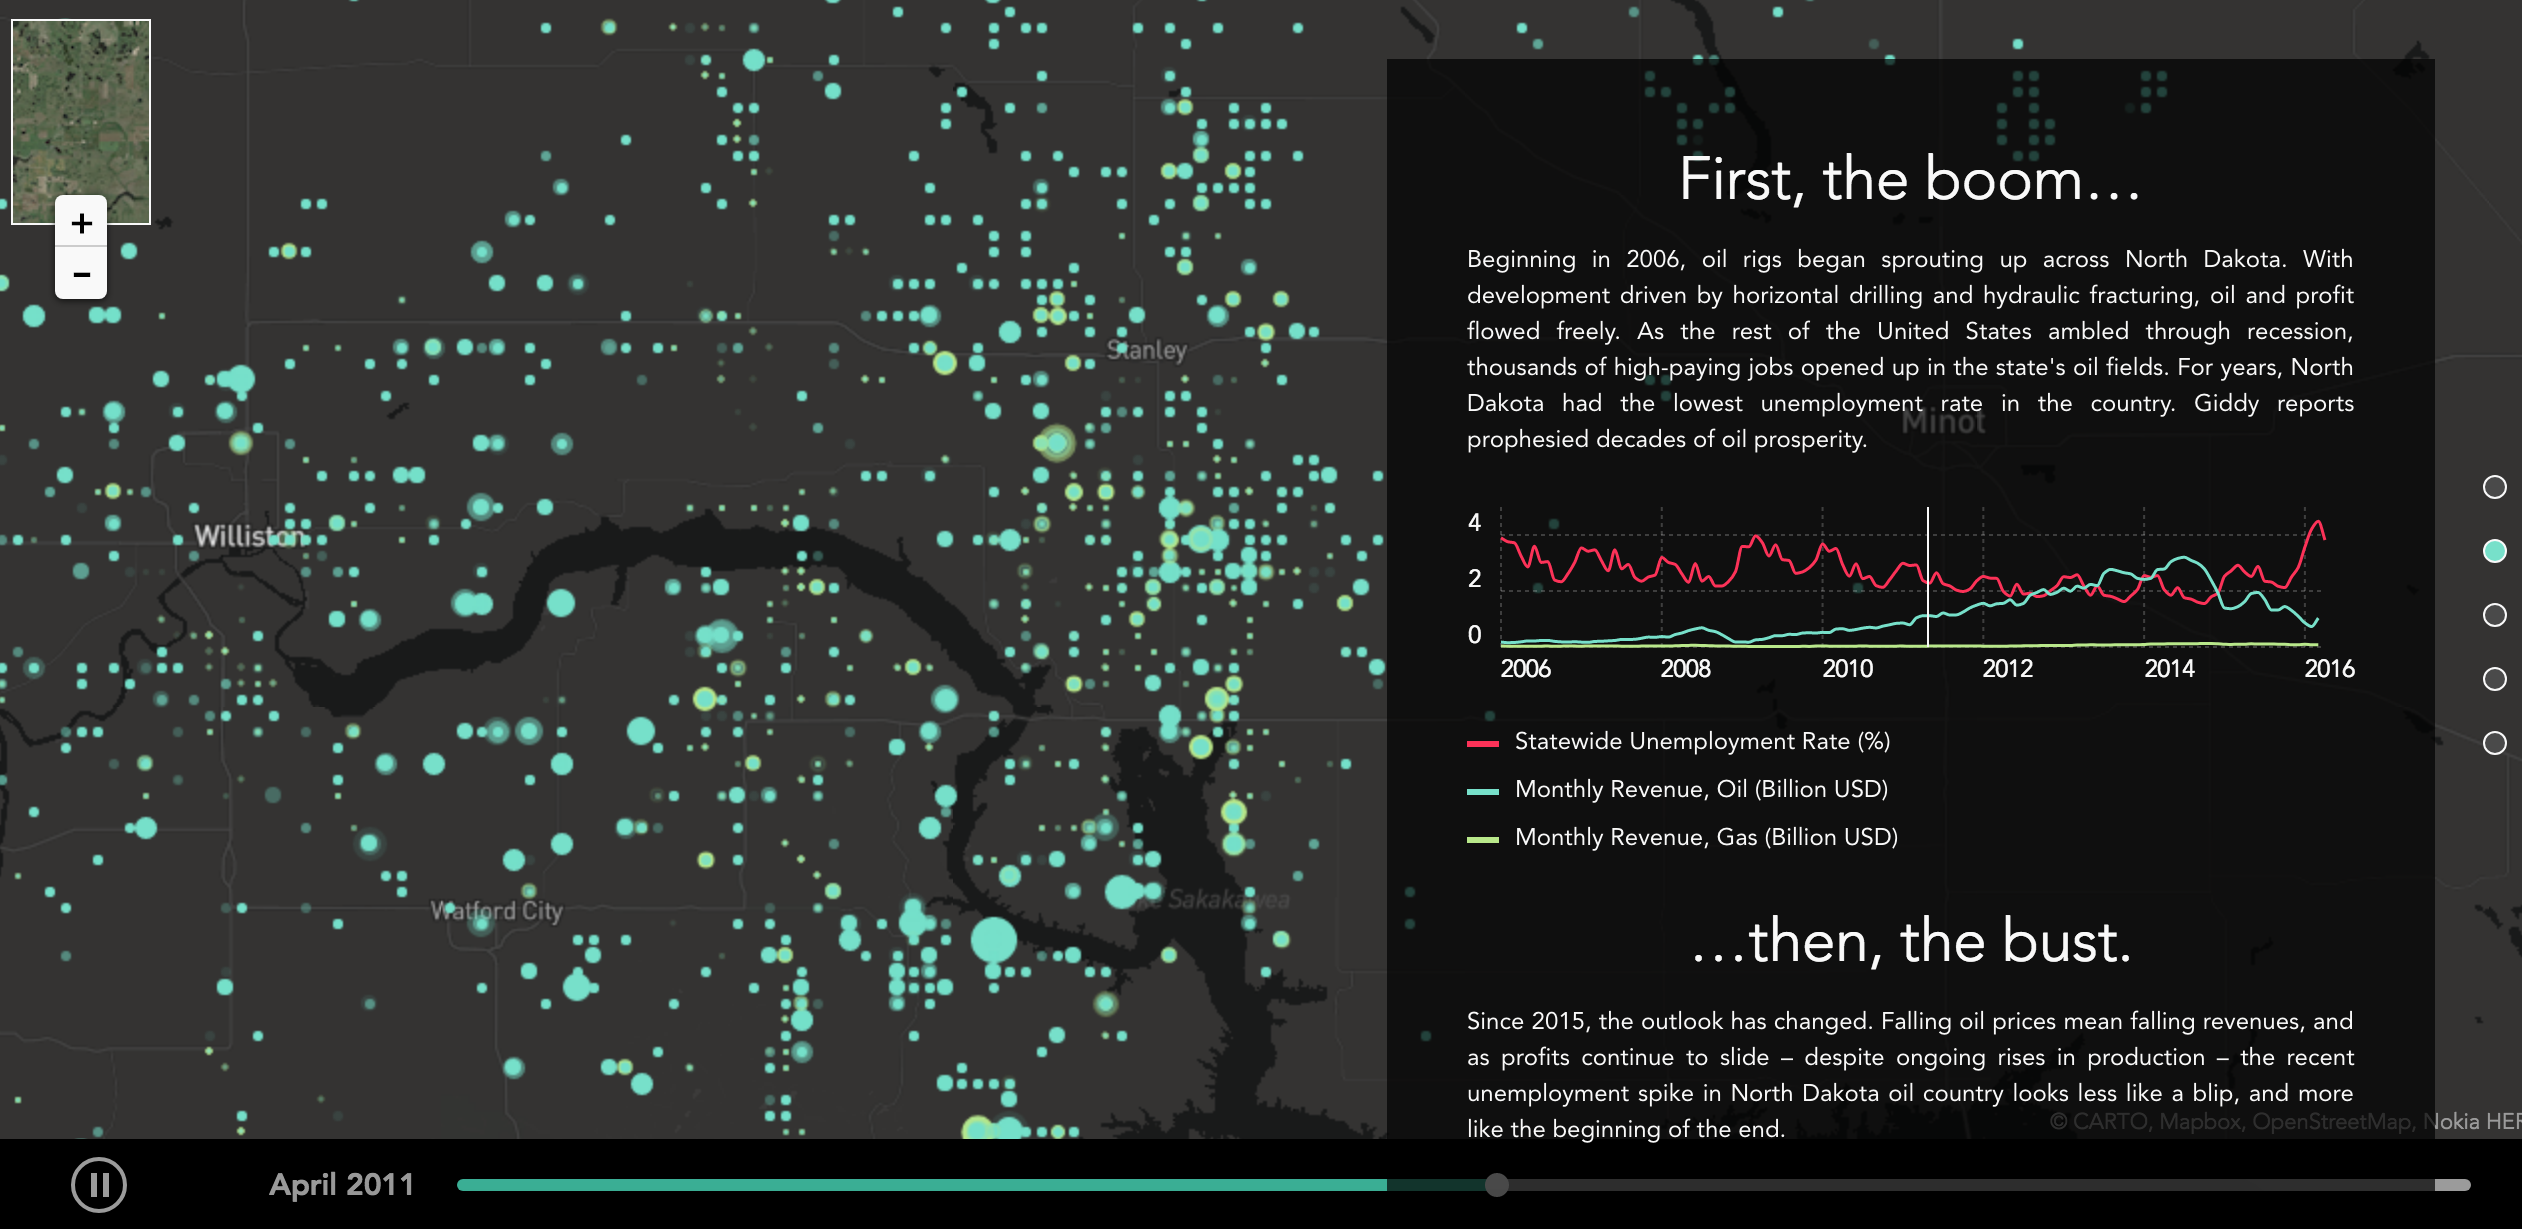
\includegraphics[width=\textwidth]{EnigmaScreenshot}
\caption{Enigma Labs North Dakota project: Historical trends show sharp increases in unemployment state-wide, with the crash in oil prices. Screenshot from https://labs.enigma.com/north-dakota-boom-to-bust/.}
\label{fig:enigma_labs}
\end{figure}

\section{Problem: US states and counties deeply dependent on fossil fuel production}

Typically, the debate over fossil fuel usage revolves around climate change issues. However, fossil fuels continue to be an important part of the US economy. Energy independence is one of the top goals for the current US administration, and was one for the last administration as well. 

Different parts of the country depend on fossil fuel production in different ways - for some states and counties, it is their primary source of livelihood. When the oil price drops, people living in these areas can be very adversely affected. In other states, for example in New York, fossil fuels are not that important to the economy, except as a commodity to be used.

The hypothesis I am working with is that many counties and states around the US continue to be deeply dependent on fossil fuel production and use. A starting point for this was the Enigma Labs project: Enigma Labs: Boom to Bust. This project centered around the effects of the oil price crash on North Dakota, and correlated the price crash with the unemployment rate in the state.

The Enigma Labs project paints a very stark picture of North Dakota's dependence on oil prices. North Dakota was one of the main beneficiaries of the US shale revolution in the 2000s. Starting in 2006, oil production in the state rapidly ramped up, leading to huge oil revenues and falling unemployment. However, with the oil price crash in 2015, this trend sharply reversed. As shown in Figure \ref{fig:enigma_labs}, there was a very sharp increase in unemployment statewide with the recent crash in oil prices. Additionally, the unemployment is also compared with oil production in the state. 

Though the original project does not really show any conclusions, it paints the shale boom in a grim light - even though there were temporary benefits, they all disappeared with the oil price crash. In this project, I delve deeper into the data, and try to see if this is indeed true for other major oil-producing counties in the US. In general, this project does not find a very clear answer. If one looks at historical data, some US counties have had real and long lasting benefits from increases in oil production. In the case of the Presidio county in Texas, the unemployment rate came down from around 40\% down to 10\%. However, oil price fluctuations do cause unemployment rates in these individual counties to fluctuate.

The most important part of this problem is trying to answer the question on how the US, and subsequently the world, will manage a transition to a carbon-free, or carbon-neutral economy. With the rapid advances being made in battery technology and electric cars, these questions affect the futures of more than a few entrepreneurs. With this project, I am trying to guess what could happen to a subset of the US economy.

\section{Target audience}

As is evident from the study on North Dakota, oil price crashes deeply impact unemployment rates in states which are the most dependent on fossil fuels. The same is true for other kinds of fossil fuels like coal and natural gas. The first obvious application of such a project would be for planning a state or county's budgets around these outcomes. So individual state governments, and/or local area authorities could be clients.

There are many other industries which indirectly are affected by the fortunes of the fossil fuel industry - since everyone relies on availability of cheap energy. These include, and are not limited to transportation, infrastructure, and manufacturing. Investors in these industries, analysts looking for exposure of companies to these sectors or just government regulators could also be potentially interested in this project.

\section{Dataset}

This project combines data from multiple sources:
\begin{enumerate}
\item Historical oil and gas production data
\item Historical oil prices (averaged monthly)
\item Local area unemployment rates and labor force numbers
\item S\&P 500 index
\end{enumerate}

Data for 3 different states was considered here: Texas, North Dakota and Wyoming. These three states are the highest oil and gas producers in the country, with Texas being the largest. North Dakota and Wyoming have both benefited from the shale boom.

The sources for each data type, and the procedure for data wrangling each of them is discussed below.

\subsection{Historical oil and gas production data}

Historical oil and gas production for all three states mentioned was gathered into csv files. This project aims to look at trends county-wise, so it was essential that the production data had county information in it. Oklahoma is actually another very high producer of oil and gas, but the Enigma data set for Oklahoma had incorrect well API numbers, so one cannot assign county information from it. The three states considered had good historical data, though it was a bit challenging to group it by county.
 
 For Texas, the Railroad Commission (RRC) provides historical oil and gas data. However, this is not trivial to extract from their website, even though it is supposed to be free. Here, the Enigma website proved to be very helpful. They also do not have the Texas data on their website, but they were willing to provide me with the raw data. Their raw data included a file containing historical oil and gas production grouped by county, which is what I used here. Unfortunately, this file does not contain data for 14 out of 254 counties, as I have explained later.
 
For both North Dakota and Wyoming, the production data is reported by individual well. There are thousands of these wells, so grouping them by county is actually good for looking at local area trends for other applications as well. Each well is identified by a unique API number (API stands for American Petroleum Institute). The first 5 digits of the well API identify the state as well as the county number, and one can look up the county name using this. The accompanying data wrangling Jupyter notebook does this for each state.
 
\subsection{Unemployment data}
The Bureau of Labor Statistics (BLS) provides local area unemployment data for the past several decades. Getting data from their website is not straightforward. From their website, one can download it by county and year, one by one, but for the large number of years I was interested in, this was too tedious and time consuming. The BLS provides a public data API, and I wrote my own code using that.

The API also does not allow extraction of more than 50 counties at a time, and more than 20 years at a time. Texas for example, has 254 counties. So one has to take this factors into account while getting the data together. The nice thing about BLS data, unlike the oil and gas production data, is that it is very well maintained and clean. However, there are some other issues with unemployment data - for example, the way `unemployment rate' is defined is a bit controversial. Typically, a lot of unemployed people are not reported in the rate if they are not actively seeking unemployment benefits, or some business has not reported layoffs. In addition, some counties in these states have a very low population compared to others. It is not very fair to compare a 10\% unemployment rate in a county with 5000 people with the same rate in a county with a million people. 

Therefore, I have collected both the unemployment rate and the labor force numbers using the BLS API, and both are taken into account while studying trends.

\subsection{Oil prices}

The historical oil price by month was downloaded from the Energy Information Administration (EIA) website. Though they have an API, it is more straightforward to just download it as a csv file. The oil price is reported daily - so for comparing it against the other kind of data, I averaged oil prices monthly.

\subsection{Macroeconomic indicators - the S\&P 500 index}

The S\&P 500 index provides a rough indicator of the wider macroeconomic health of the economy. This is important as often a sharp rise in unemployment accompanied by oil price crashes is actually the result of a wider economic recession. Therefore, to delineate these effects, I have also collected S\&P 500 data from http://www.cboe.com/micro/buywrite/dailypricehistory.xls. Similar to the oil price, the S\&P data needed to be averaged monthly.

\begin{figure}
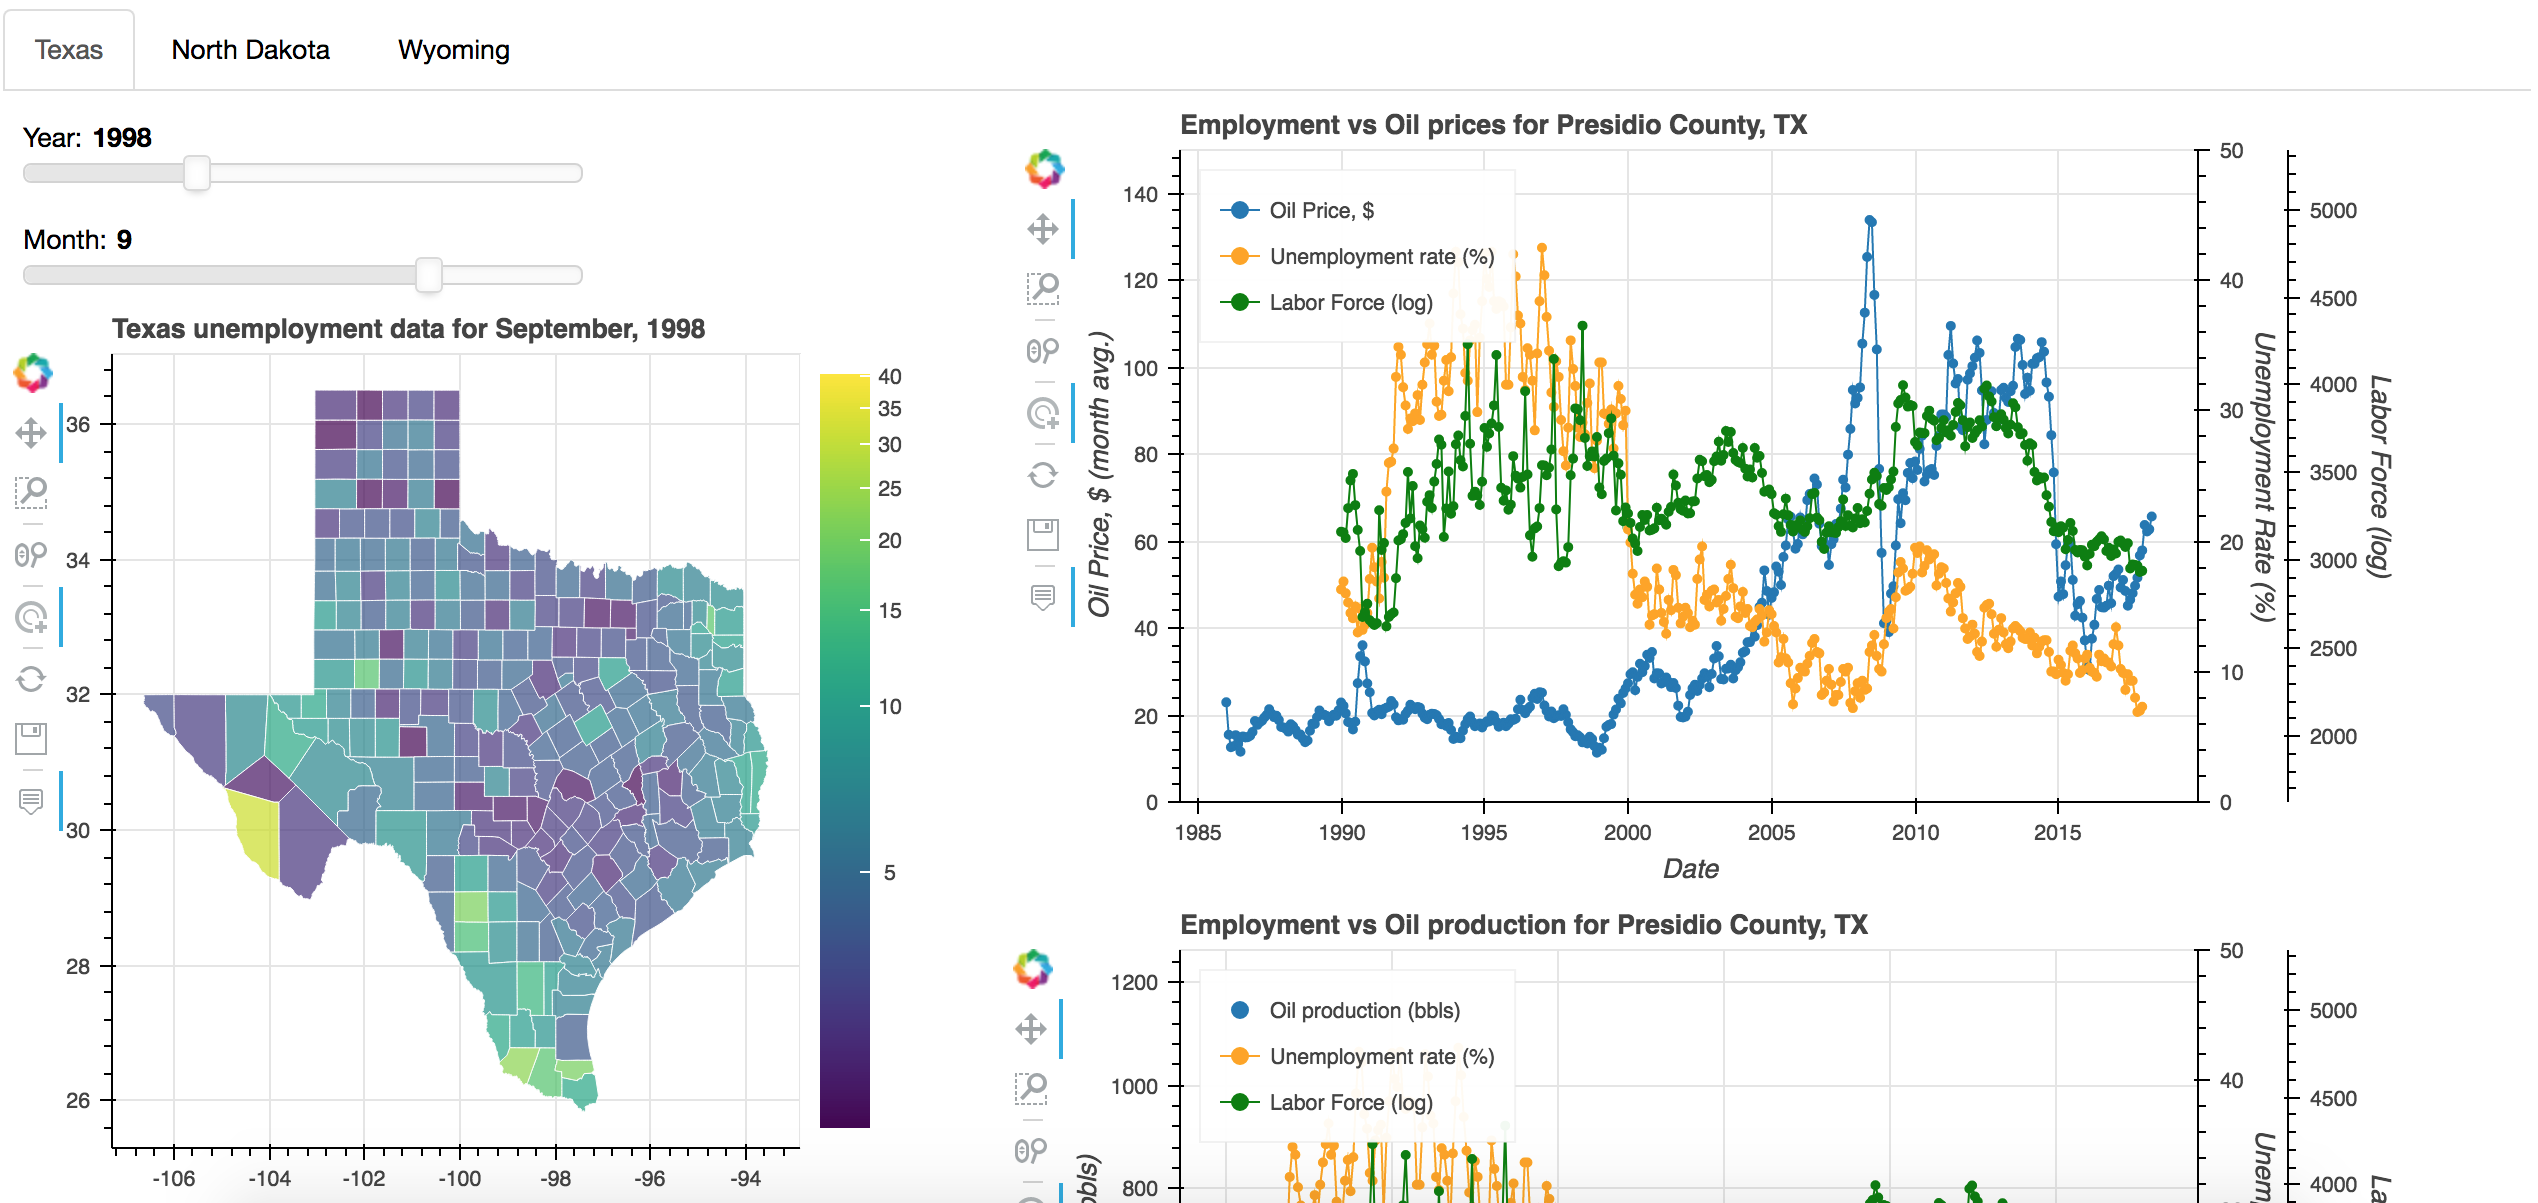
\includegraphics[width=\textwidth]{BokehAppScreenshot}
\caption{Screenshot of the Bokeh app created to visualize historical county data for 3 states. Different kinds of data include county unemployment rate,  county labor force, county oil production, S\&P 500 index, and oil prices. The app includes sliders to vary the year and month, and clicking on a particular county reveals the entire historical data for that county.}
\label{fig:bokeh_app}
\end{figure}

\section{Exploratory data analysis}
For this section, I put together the different data sources, combining it into visualizations, for all three states. For this purpose, I created a Bokeh app, which made it easy to change the year and month, and to visualize changes in oil and gas production, and unemployment. Bokeh also provides a sample dataset which contains the boundaries of all US counties and states. Using this dataset, I was able to generate color-coded maps of all states for visualizing unemployment and oil production.

Figure \ref{fig:bokeh_app} shows a screenshot of the Bokeh app. The app can be launched from the commandline, and is currently being set up on the cloud using Anaconda's cloud hosting. Using the app, it is simpler to navigate historical trends in the different kinds of data. In the following sections, each state is explored separately, with interesting trends from individual counties highlighted.


\subsection{Texas}

Figure \ref{fig:tx_maps} shows unemployment and oil production data for all counties. Three different years are considered: 1995, 2005 and 2015, showing changes in unemployment distribution over time. The month of September is chosen for consistency across all maps. The figures show decreasing unemployment across many counties over time, while the oil production in selected counties go up. The figures for oil production do not quite capture the increase in oil production, as they are relative maps. 

Figure \ref{fig:tx_hist_data} shows examples of individual counties in Texas. Maverick county is an example of a high oil-producing county. As shown in Figure \ref{fig:tx_hist_data}, not only have unemployment levels reduced in this area, but the seasonal fluctuations in unemployment have stabilized. Going by the sharp increase in oil production, this stability can be safely attributed to increased oil revenues in the area. On the other hand, Val Verde county produces very little oil. This area is not affected much by fluctuations in oil prices, though wider economic recessions do affect it.

\begin{figure}
\centering
\begin{subfigure}{0.3\textwidth}
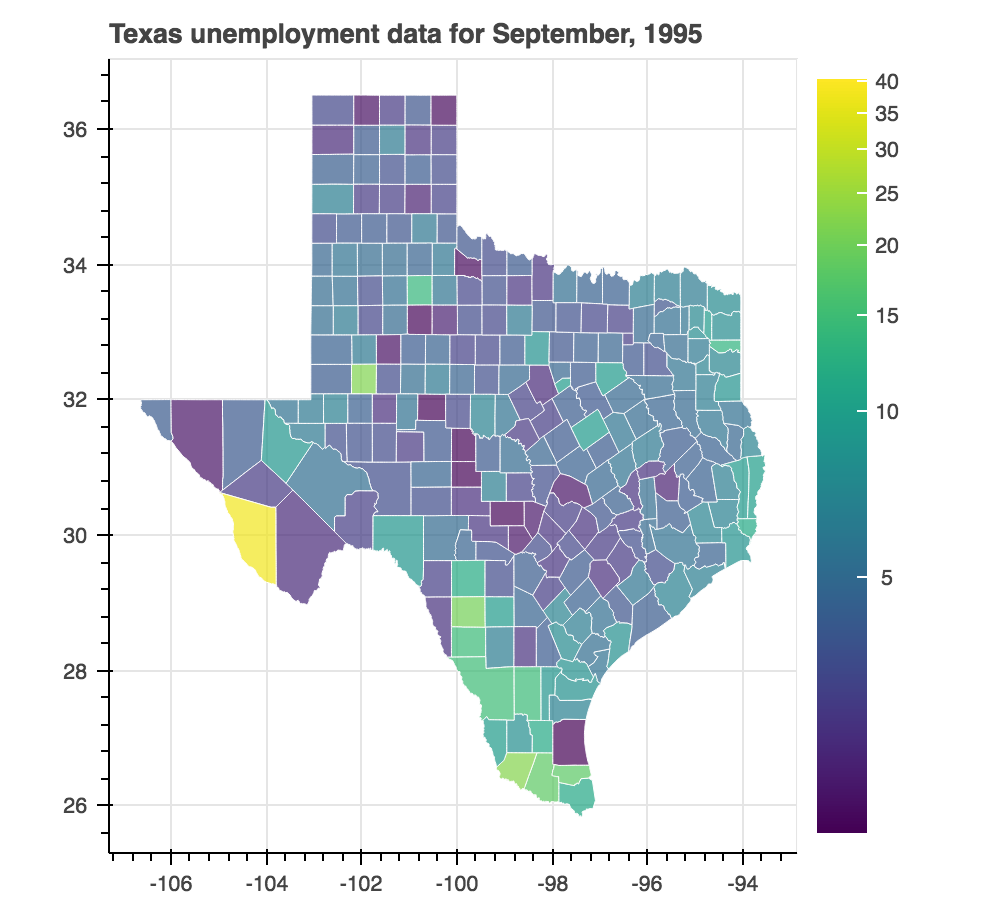
\includegraphics[width=1.2\linewidth]{tx_unemp_1995}
\end{subfigure}
~
\begin{subfigure}{0.3\textwidth}
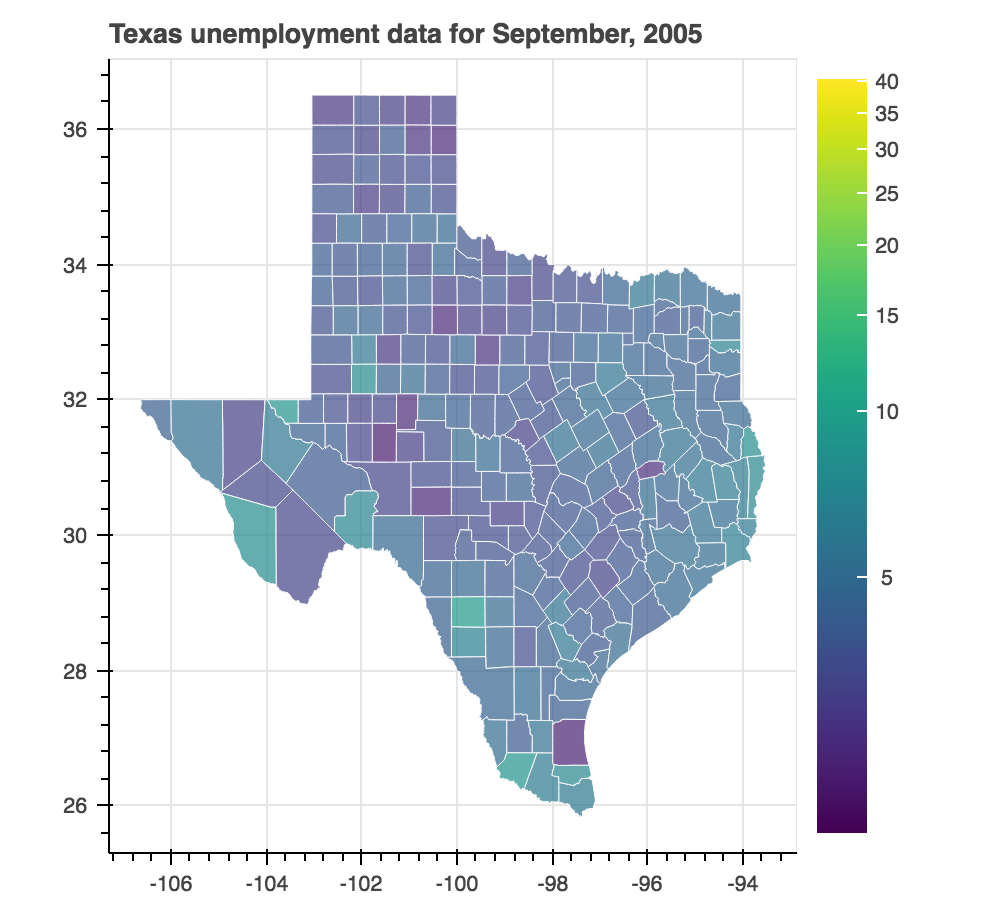
\includegraphics[width=1.2\linewidth]{tx_unemp_2005}
\end{subfigure}
~
\begin{subfigure}{0.3\textwidth}
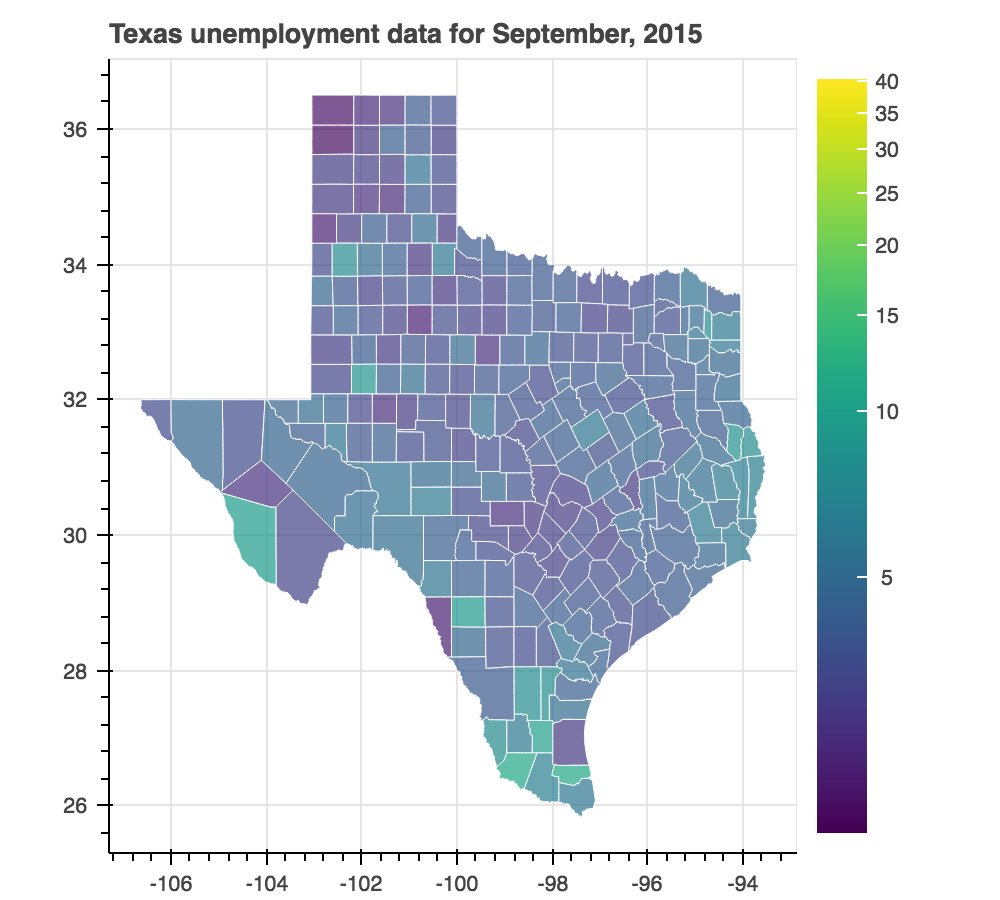
\includegraphics[width=1.2\linewidth]{tx_unemp_2015}
\end{subfigure}

\begin{subfigure}{0.3\textwidth}
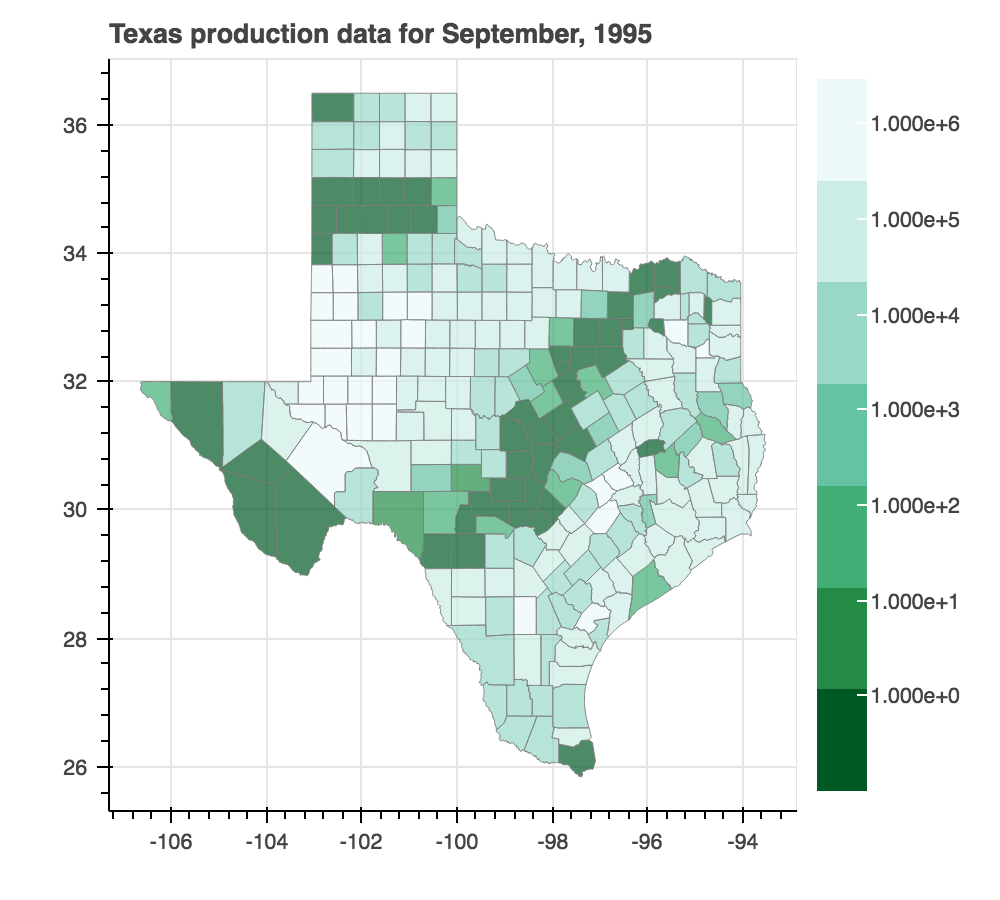
\includegraphics[width=1.2\linewidth]{tx_prod_1995}
\end{subfigure}
~
\begin{subfigure}{0.3\textwidth}
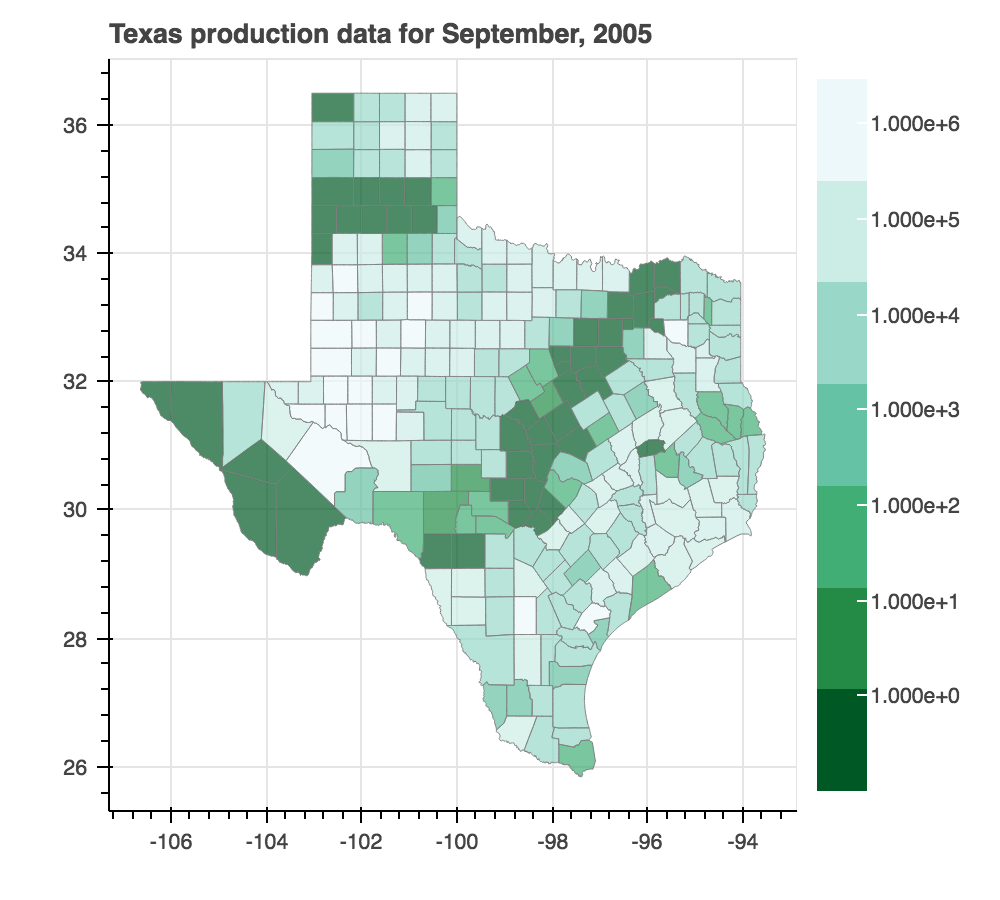
\includegraphics[width=1.2\linewidth]{tx_prod_2005}
\end{subfigure}
~
\begin{subfigure}{0.3\textwidth}
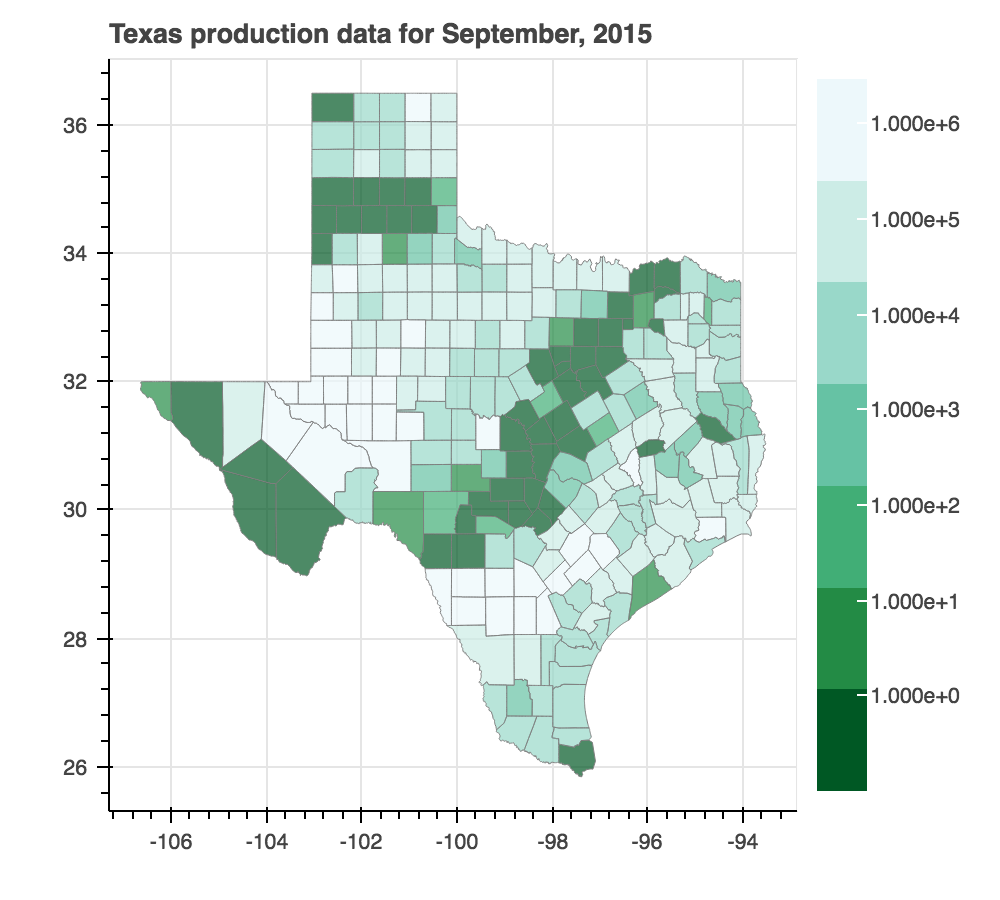
\includegraphics[width=1.2\linewidth]{tx_prod_2015}
\end{subfigure}
\caption{Texas trends: The top row shows evolution of unemployment rates in Texas from 1995-2015, while the bottom row shows oil production data. The maps show overall reducing unemployment rates in the state, along with increasing oil production in some counties.}
\label{fig:tx_maps}
\end{figure}

\begin{figure}
\centering
\begin{subfigure}{0.45\textwidth}
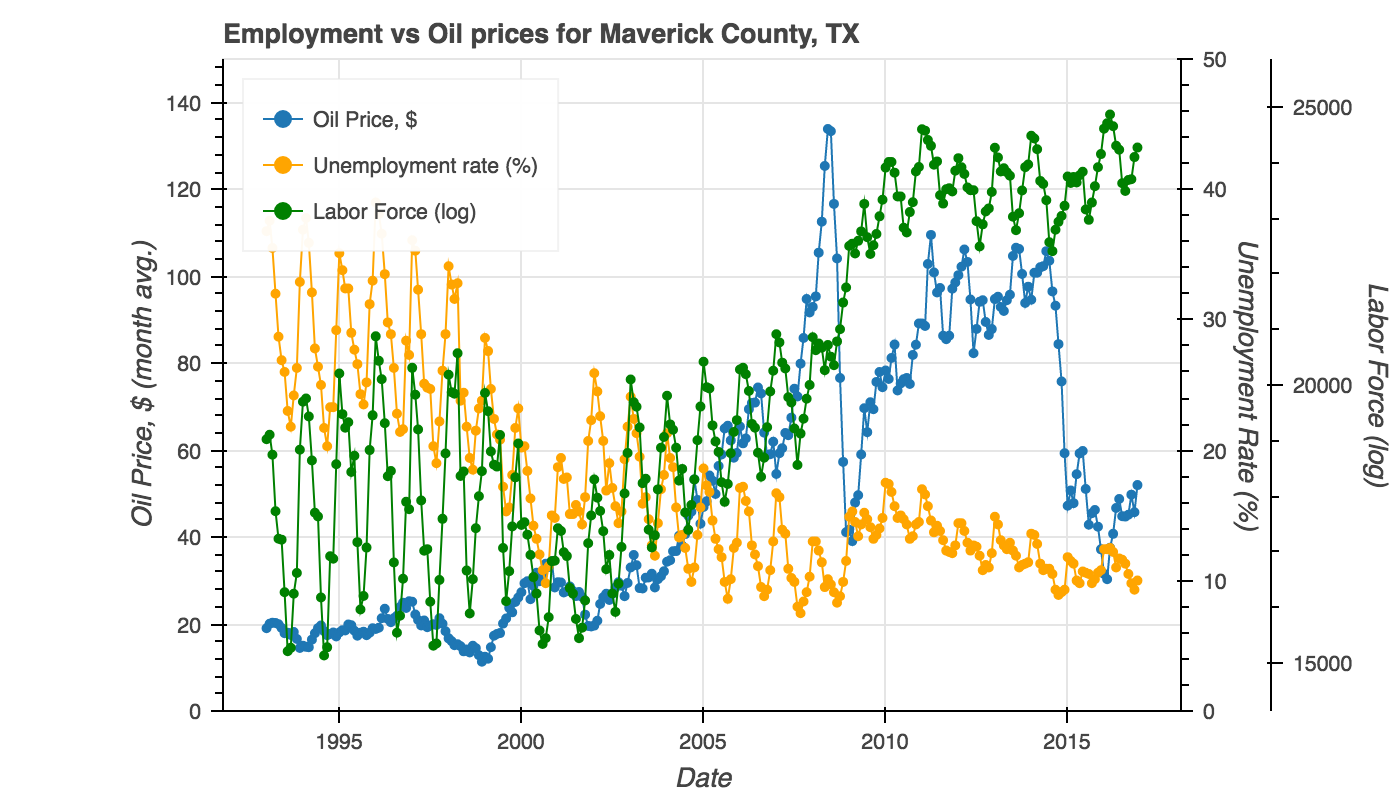
\includegraphics[width=1.1\linewidth]{tx_maverick_oil_price}
\end{subfigure}
~
\begin{subfigure}{0.45\textwidth}
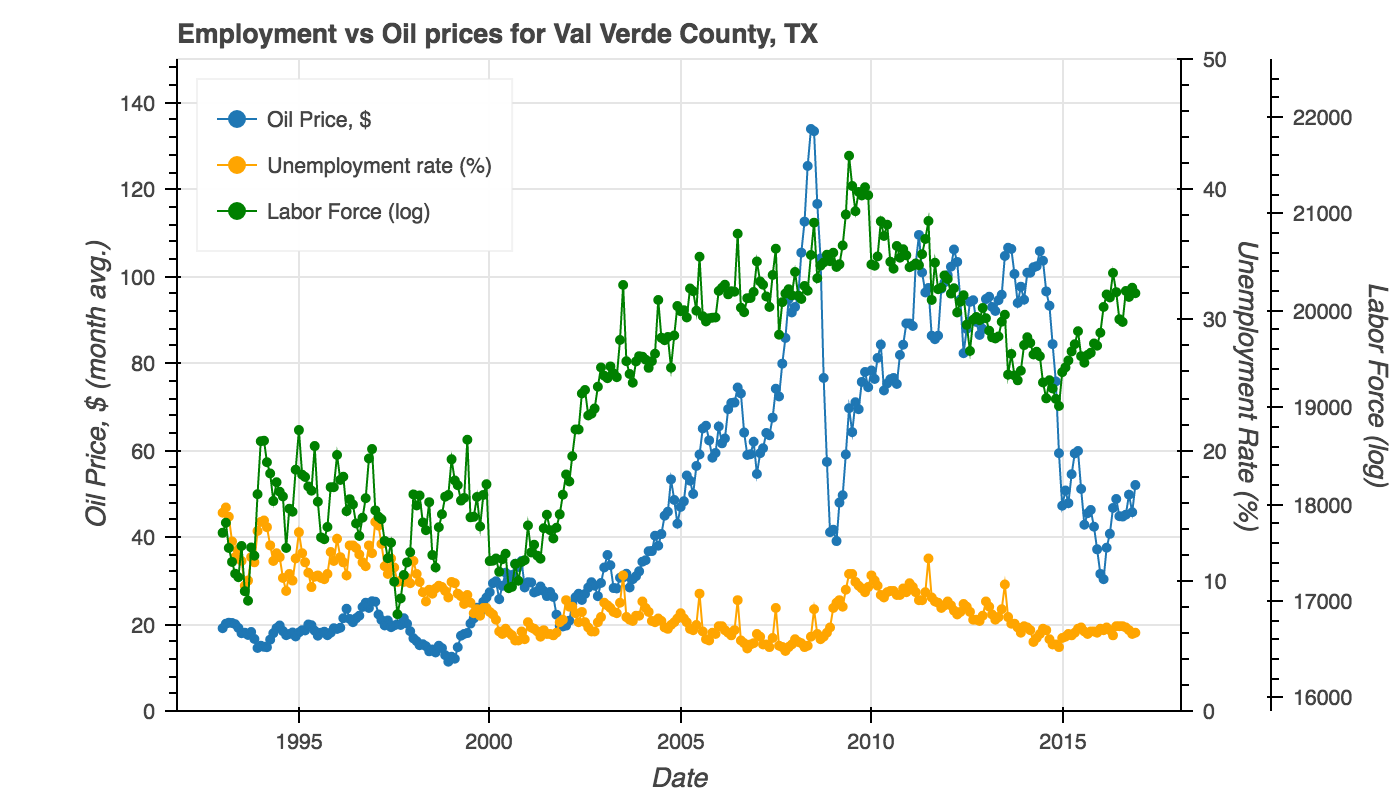
\includegraphics[width=1.1\linewidth]{tx_valverde_oil_price}
\end{subfigure}

\begin{subfigure}{0.45\textwidth}
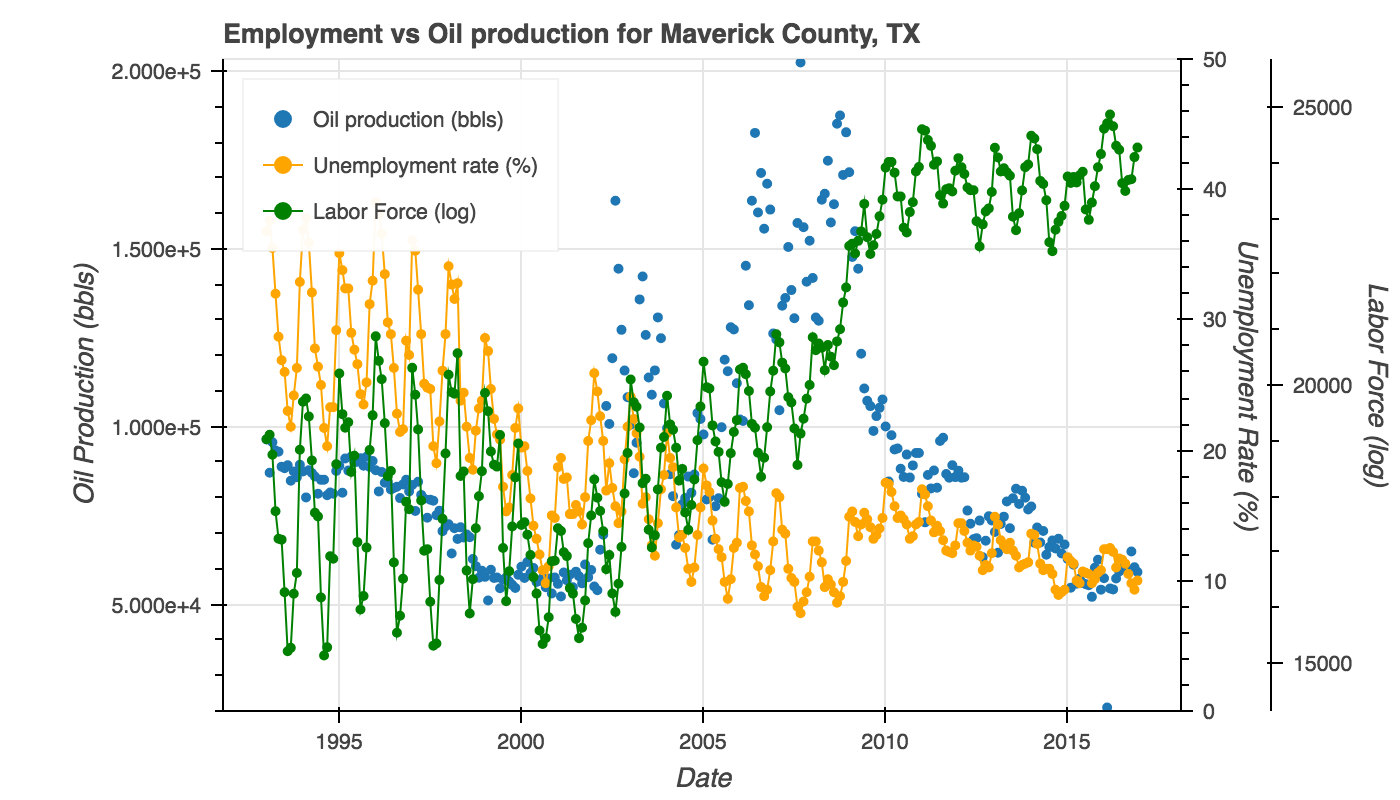
\includegraphics[width=1.1\linewidth]{tx_maverick_oil_prod}
\end{subfigure}
~
\begin{subfigure}{0.45\textwidth}
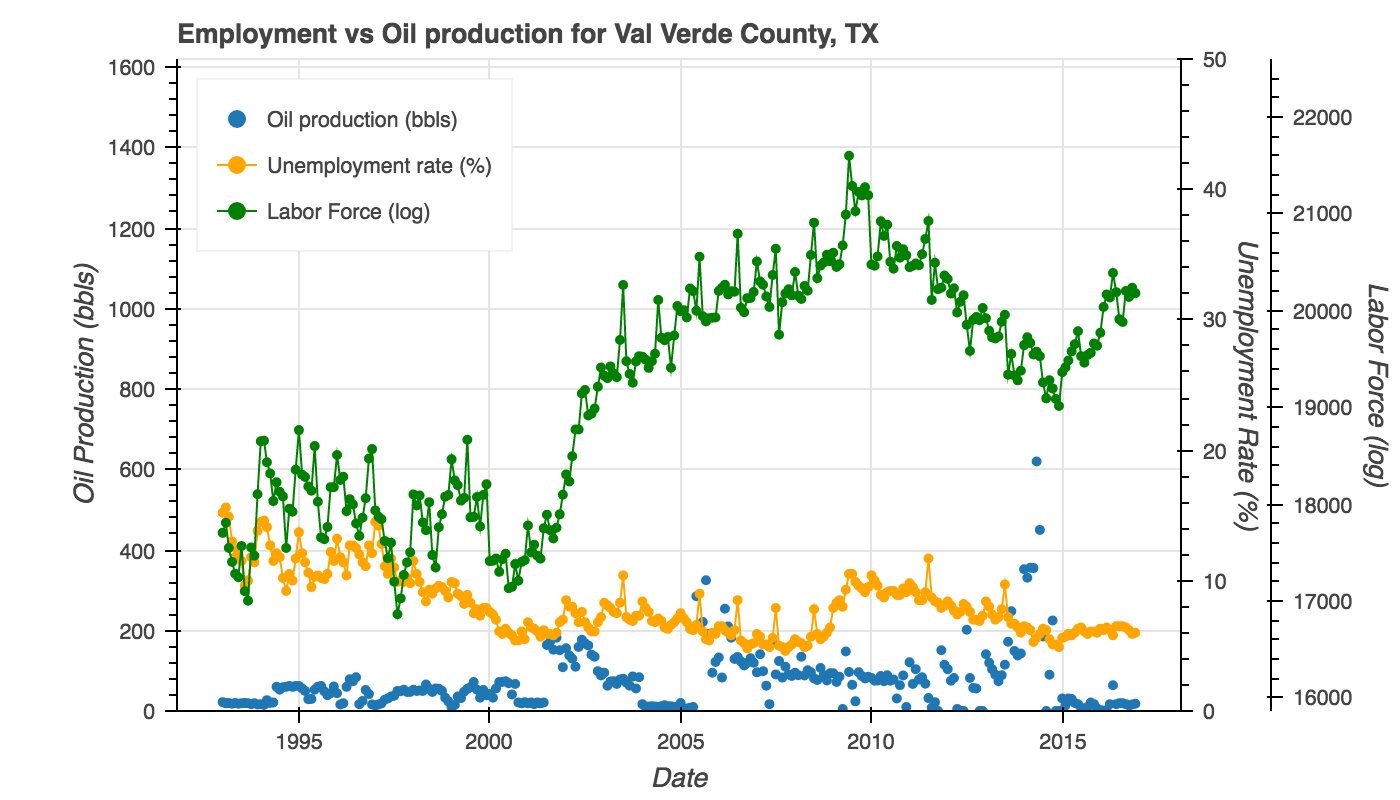
\includegraphics[width=1.1\linewidth]{tx_valverde_oil_prod}
\end{subfigure}

\begin{subfigure}{0.45\textwidth}
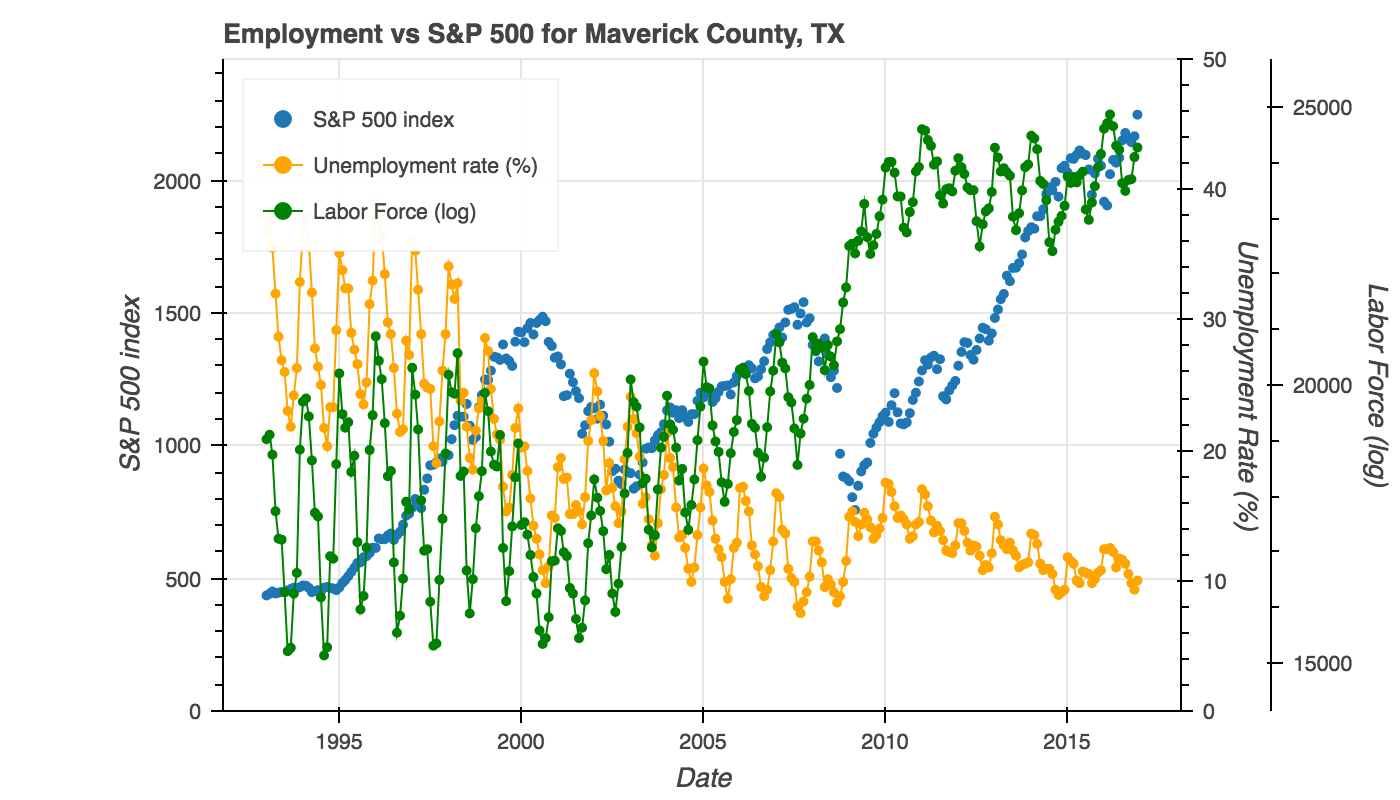
\includegraphics[width=1.1\linewidth]{tx_maverick_snp}
\end{subfigure}
~
\begin{subfigure}{0.45\textwidth}
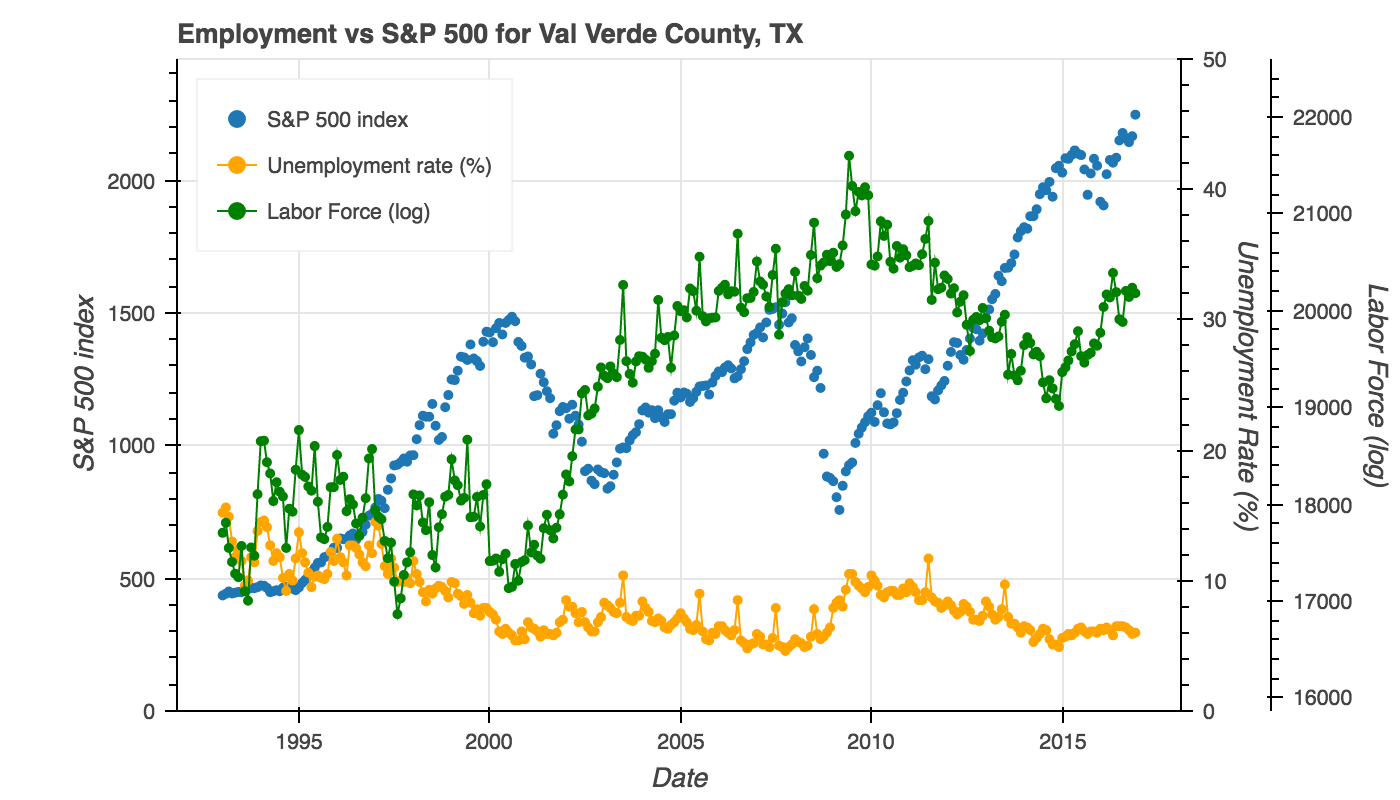
\includegraphics[width=1.1\linewidth]{tx_valverde_snp}
\end{subfigure}

\caption{The left column shows data for Maverick county, TX (a high oil producer), while the right one shows data for Val Verde county, TX (a low oil producer). Historical data for Maverick county over a 20-year period show sharp changes in unemployment rate as well as labor force in the county. As the oil production in the county rises, the sharp yearly changes in unemployment stabilize. For Val Verde county, unemployment rates in the county are not affected much over time by any one variable considered here, remaining roughly constant. There are seasonal variations, which are also affected by wider economy slowdowns, for example in the 2008 recession.}
\label{fig:tx_hist_data}
\end{figure}


\subsection{North Dakota}

North Dakota was the subject of the original Enigma Labs project. That project focused on the 2010-2015 period, and concluded that increasing oil production brought about diminishing returns for individual counties in the area. 

Figure \ref{fig:nd_maps} shows unemployment and oil production maps for North Dakota for 1995, 2005, and 2015. Looking at this data, the conclusion in the Enigma Labs' project does not seem very supportable. While it is true that oil price fluctuations have brought about corresponding fluctuations in unemployment, overall, the unemployment levels in the state have dropped. Another interesting feature of this state is that \emph{all} the oil production is concentrated in the western part of the state. The counties with little to no oil production are not affected - and there are several of them.

Figure \ref{fig:nd_hist_data} shows historical data for McKenzie and McLean counties. McKenzie county is one of the highest oil producing counties in North Dakota. Looking at its graph, the huge bump in oil production during the 2000s shale revolution is also apparent. In 2015, the year the oil price crashed, one can see a bump in the unemployment rate, however this period also saw a huge increase in the labor force in the county. Since most of the additional labor force came in because of the oil production increase, the bump is not at all unexpected. Figure \ref{fig:nd_hist_data} also shows the same data for McLean county. This is a comparatively low producing area, and the data shows negligible impact of oil prices on the county unemployment rate. There was also no increase in labor force with oil production, hence it is also clear there would be no effect on unemployment rates.

\begin{figure}[h!]
\centering
\begin{subfigure}{0.3\textwidth}
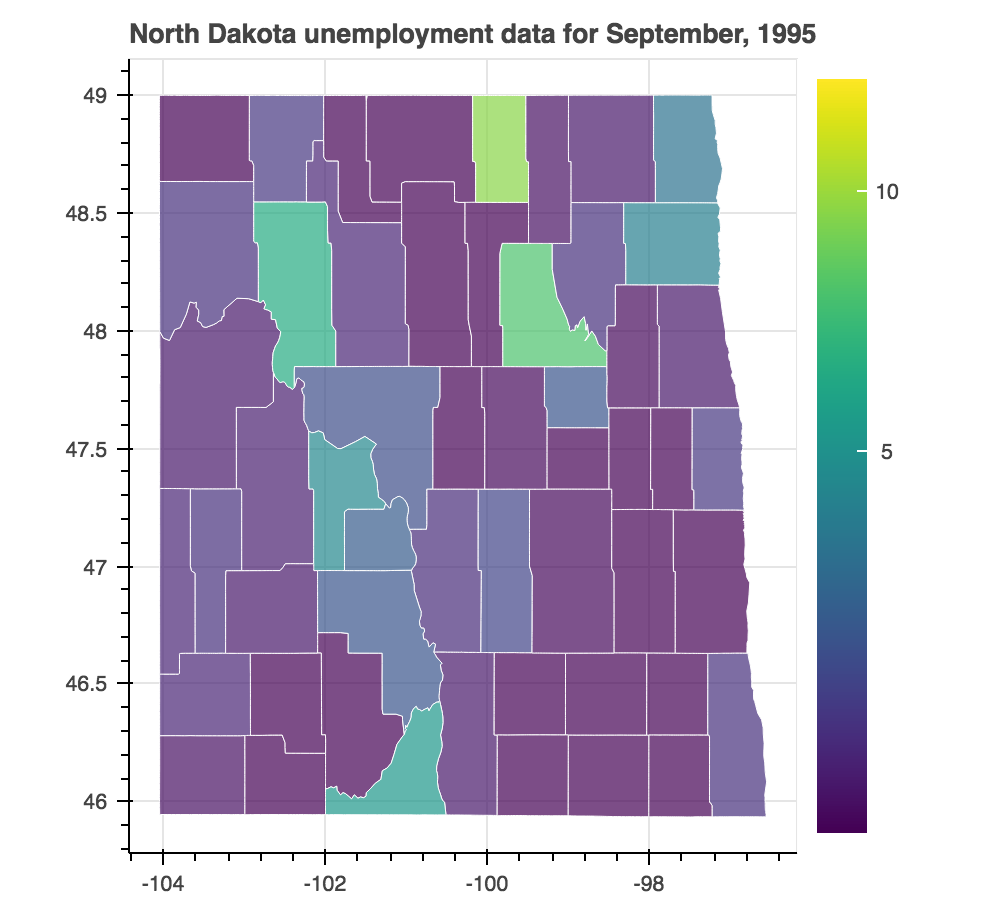
\includegraphics[width=1.2\linewidth]{nd_unemp_1995}
\end{subfigure}
~
\begin{subfigure}{0.3\textwidth}
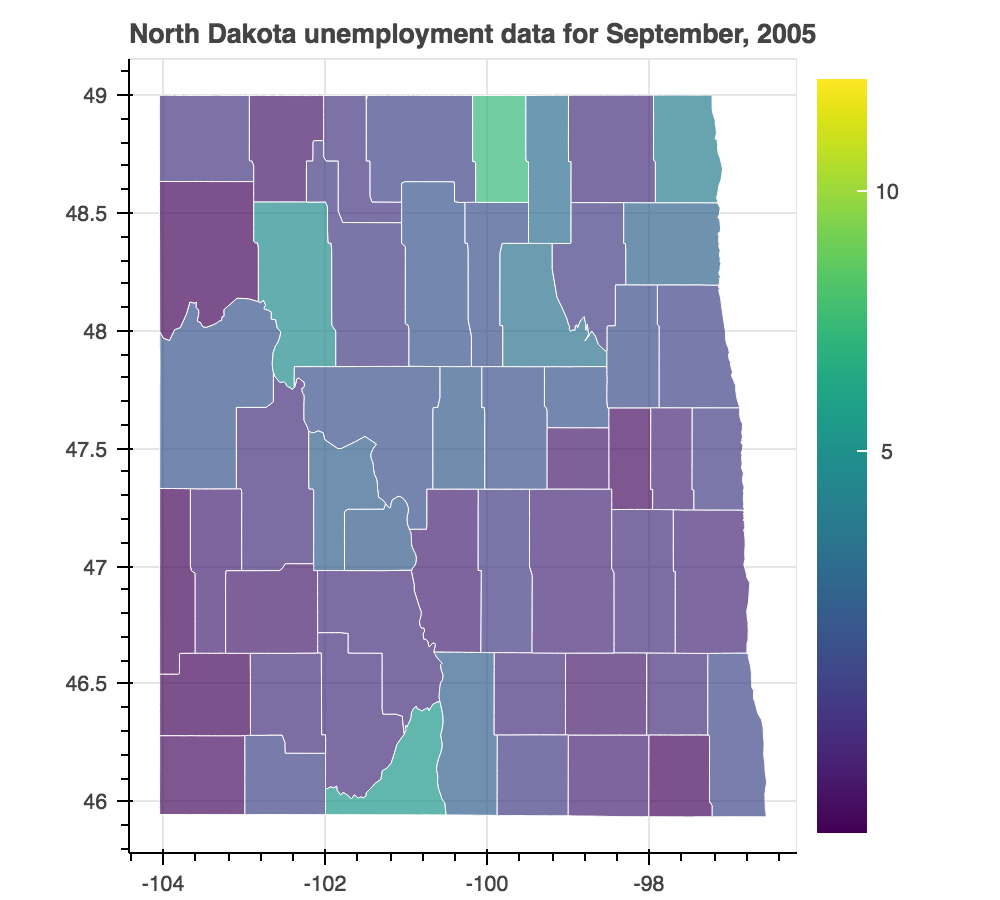
\includegraphics[width=1.2\linewidth]{nd_unemp_2005}
\end{subfigure}
~
\begin{subfigure}{0.3\textwidth}
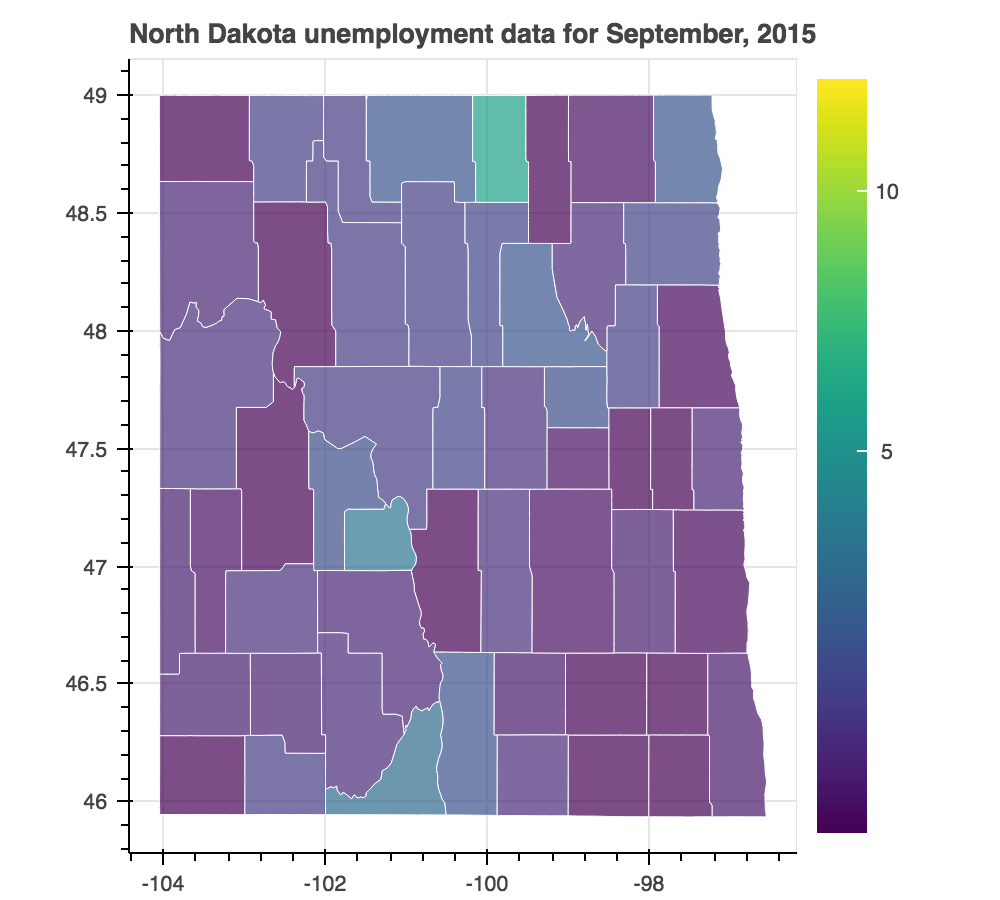
\includegraphics[width=1.2\linewidth]{nd_unemp_2015}
\end{subfigure}

\begin{subfigure}{0.3\textwidth}
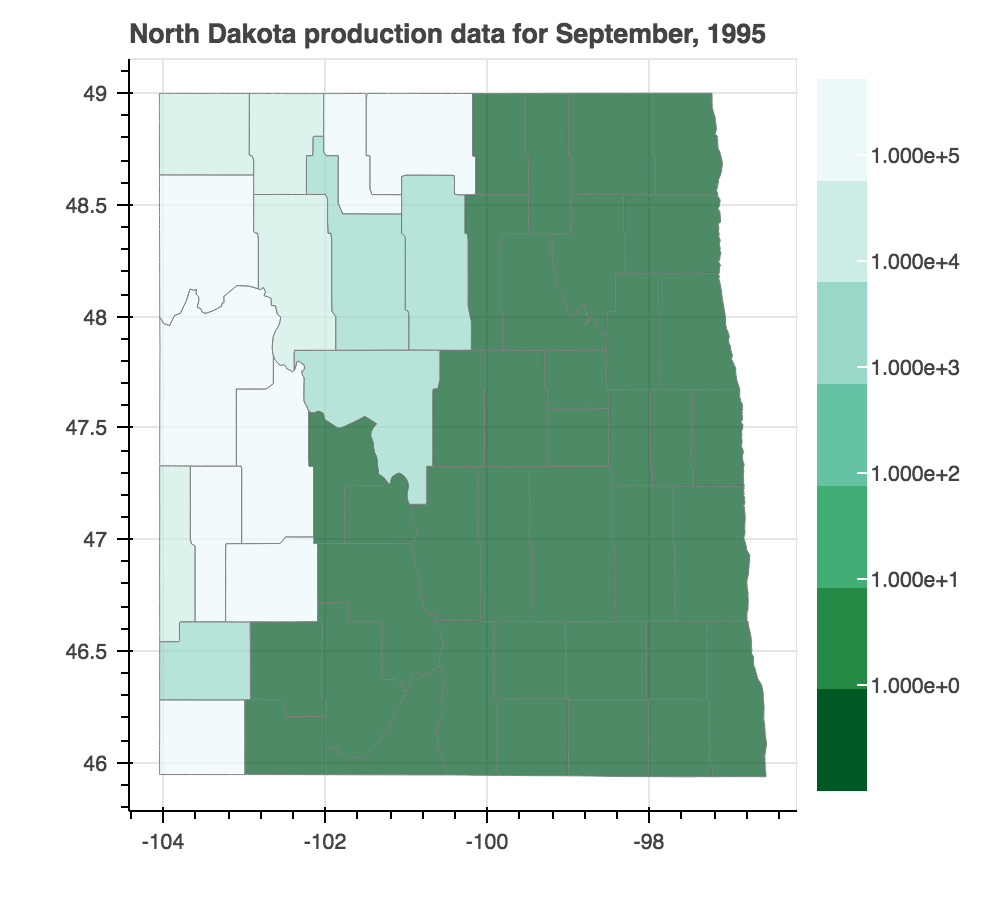
\includegraphics[width=1.2\linewidth]{nd_prod_1995}
\end{subfigure}
~
\begin{subfigure}{0.3\textwidth}
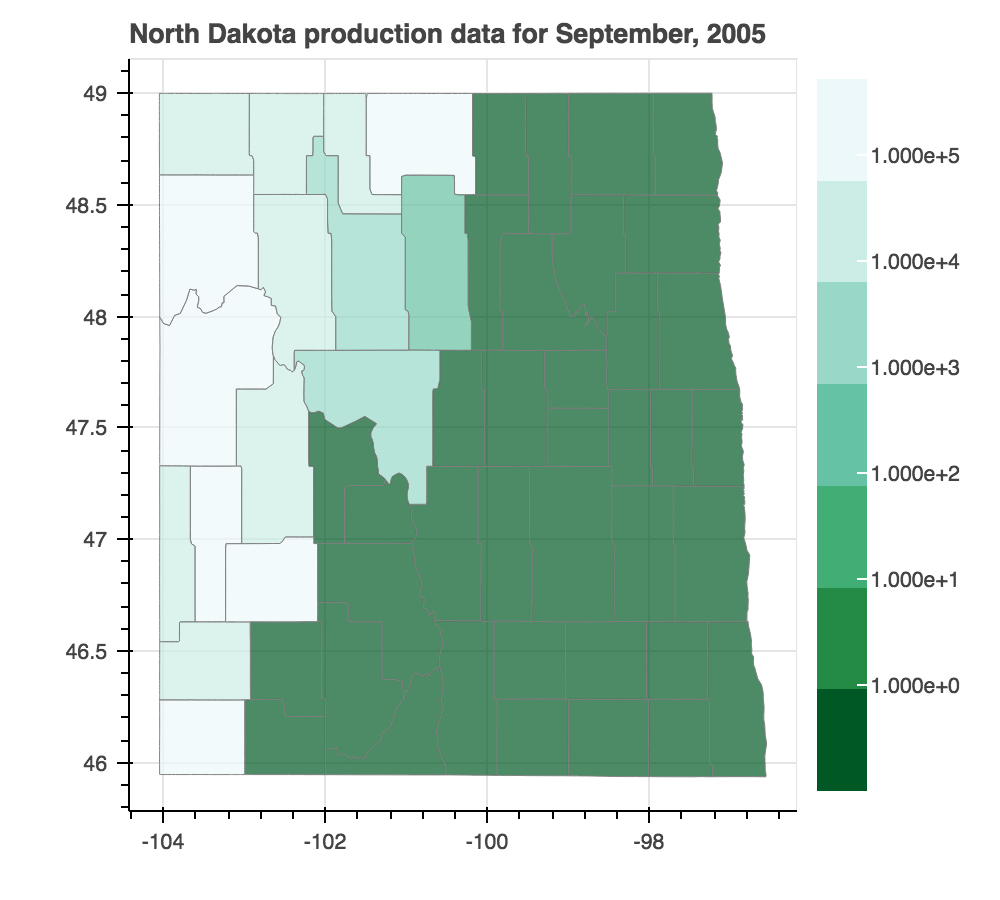
\includegraphics[width=1.2\linewidth]{nd_prod_2005}
\end{subfigure}
~
\begin{subfigure}{0.3\textwidth}
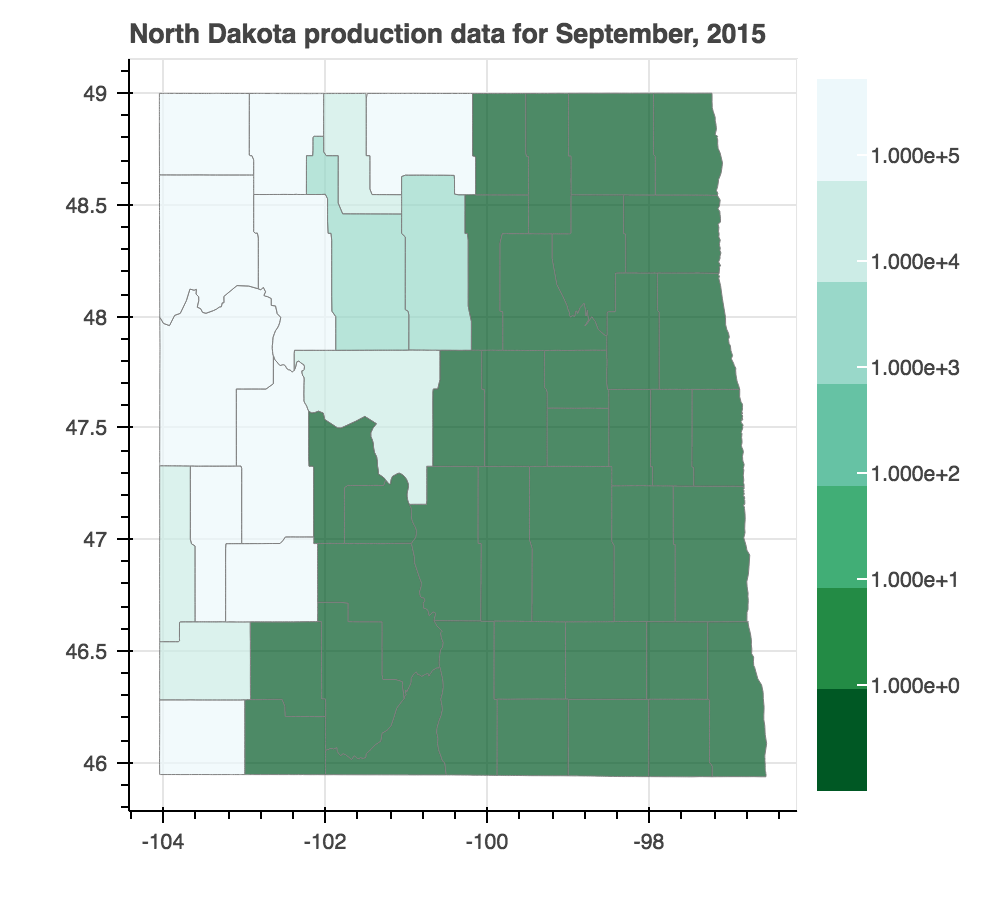
\includegraphics[width=1.2\linewidth]{nd_prod_2015}
\end{subfigure}
\caption{North Dakota trends: The top row shows evolution of unemployment rates in North Dakota from 1995-2015, while the bottom row shows oil production data. Similar to Texas, the unemployment levels in the state have decreased overall. However, most of the dramatic increases in oil production have come in counties which were already significant oil producers, so they do not show up in the colored maps. }
\label{fig:nd_maps}
\end{figure}

\begin{figure}
\centering
\begin{subfigure}{0.45\textwidth}
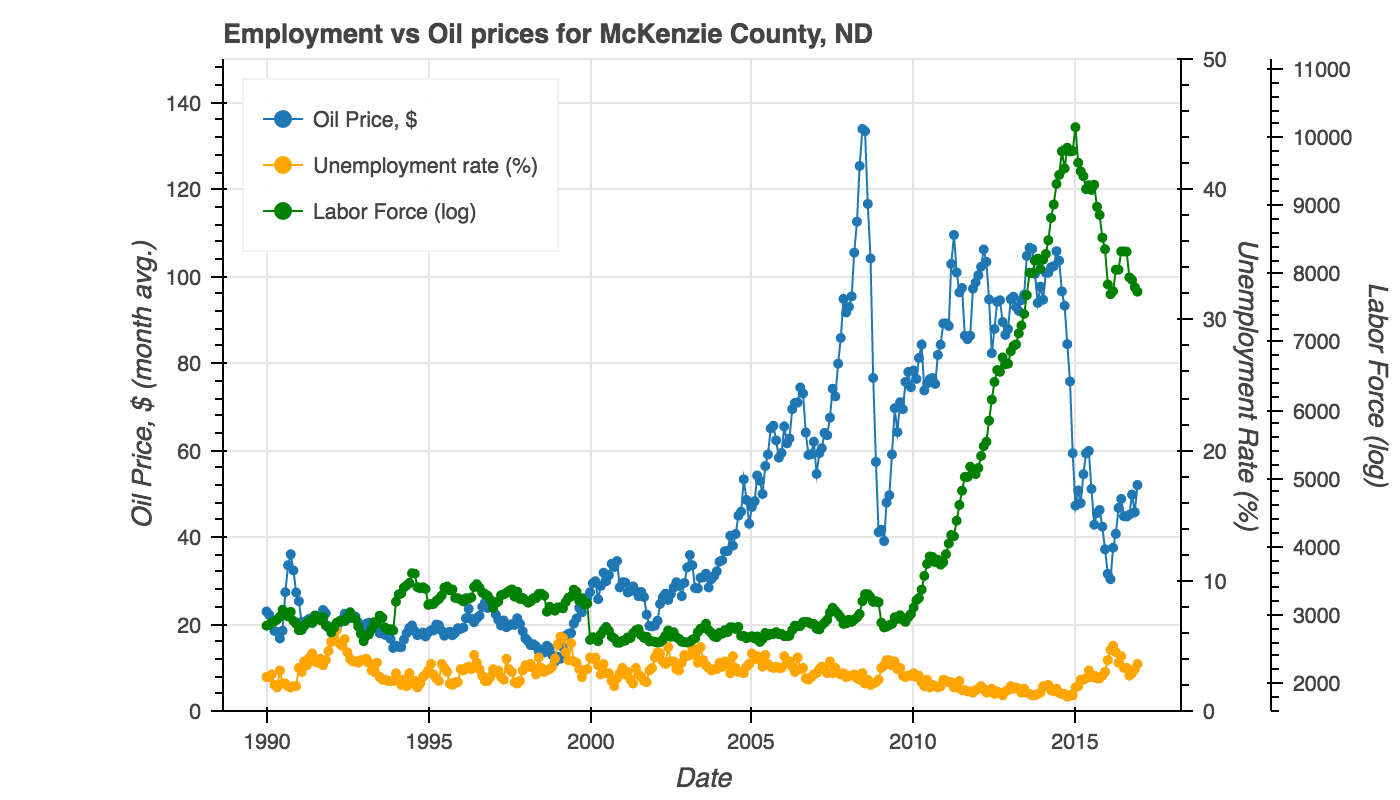
\includegraphics[width=1.1\linewidth]{nd_mckenzie_oil_price}
\end{subfigure}
~
\begin{subfigure}{0.45\textwidth}
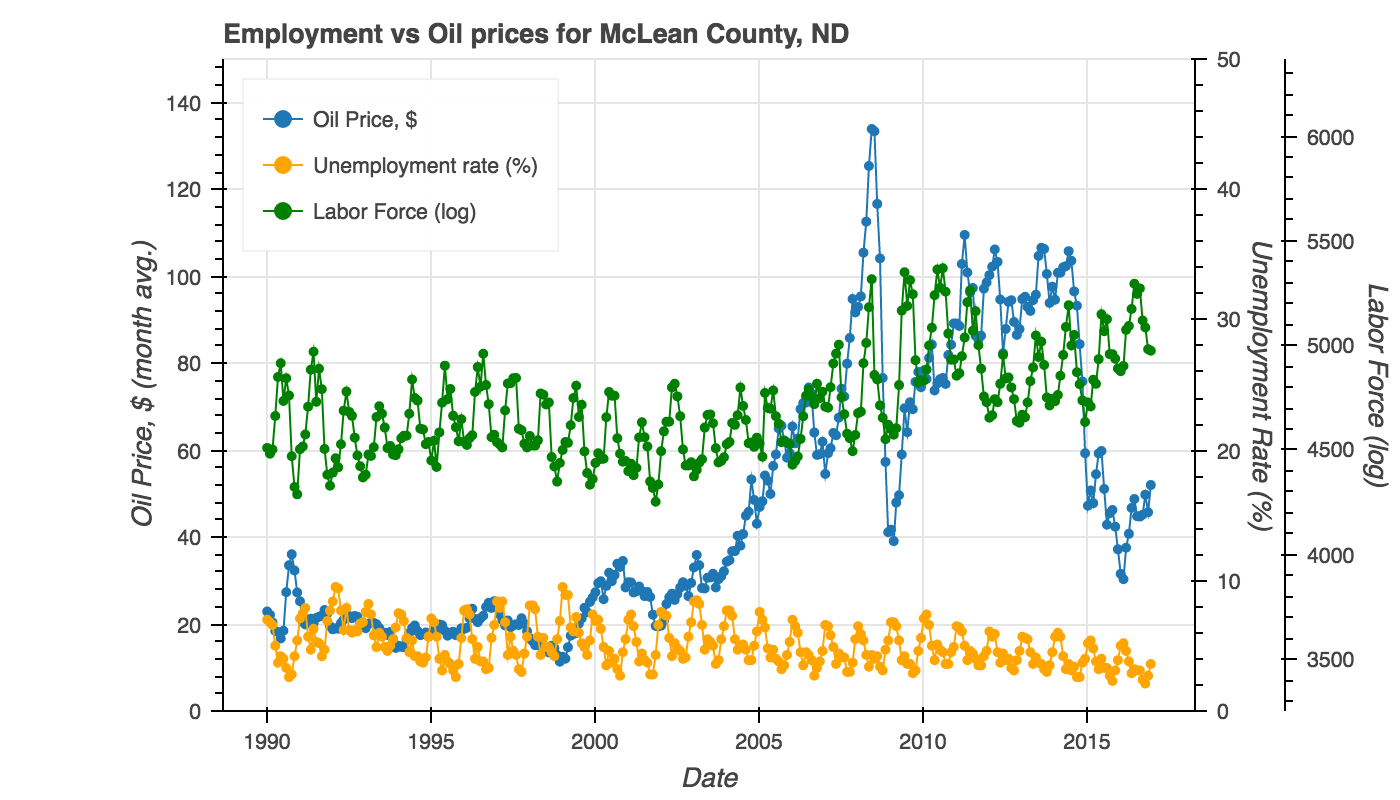
\includegraphics[width=\linewidth]{nd_mclean_oil_price}
\end{subfigure}

\begin{subfigure}{0.45\textwidth}
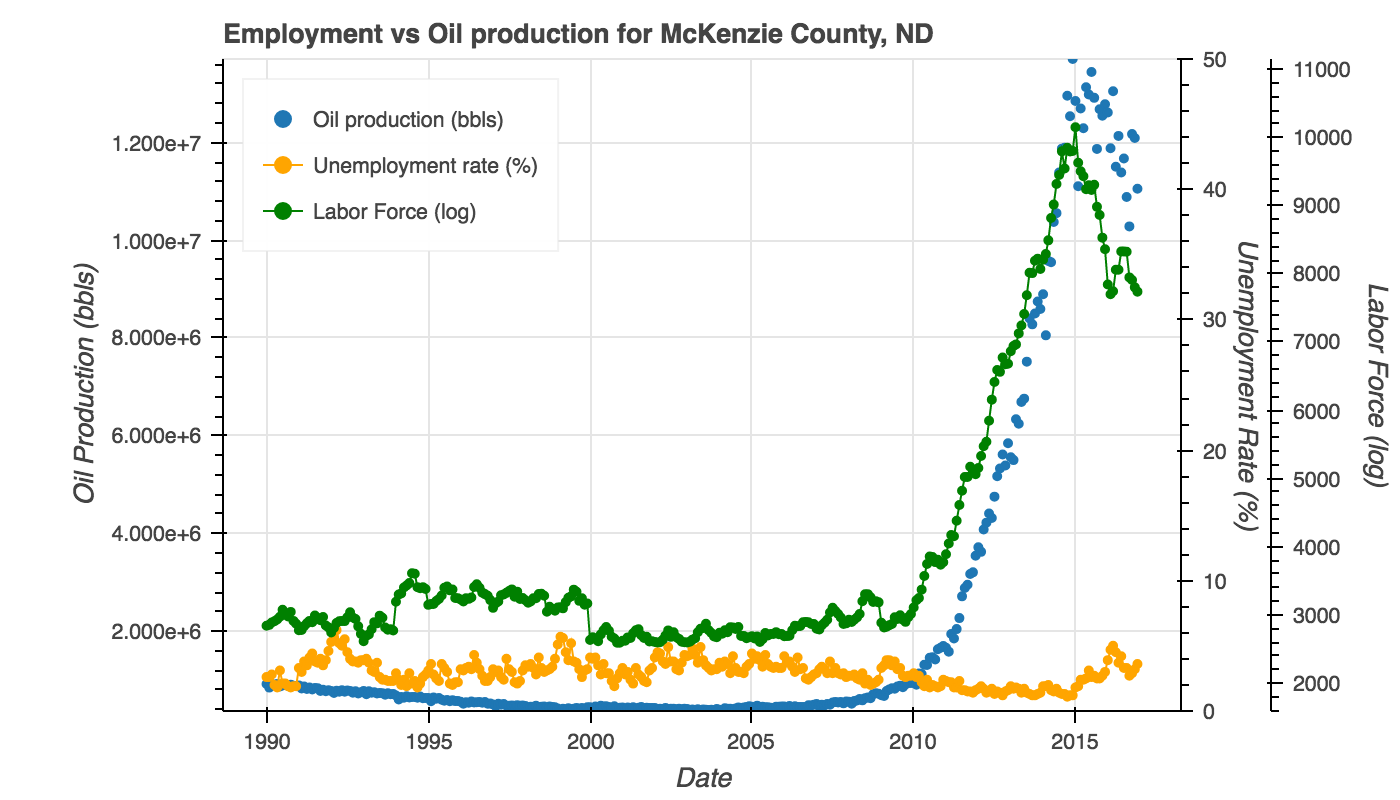
\includegraphics[width=1.1\linewidth]{nd_mckenzie_oil_prod}
\end{subfigure}
~
\begin{subfigure}{0.45\textwidth}
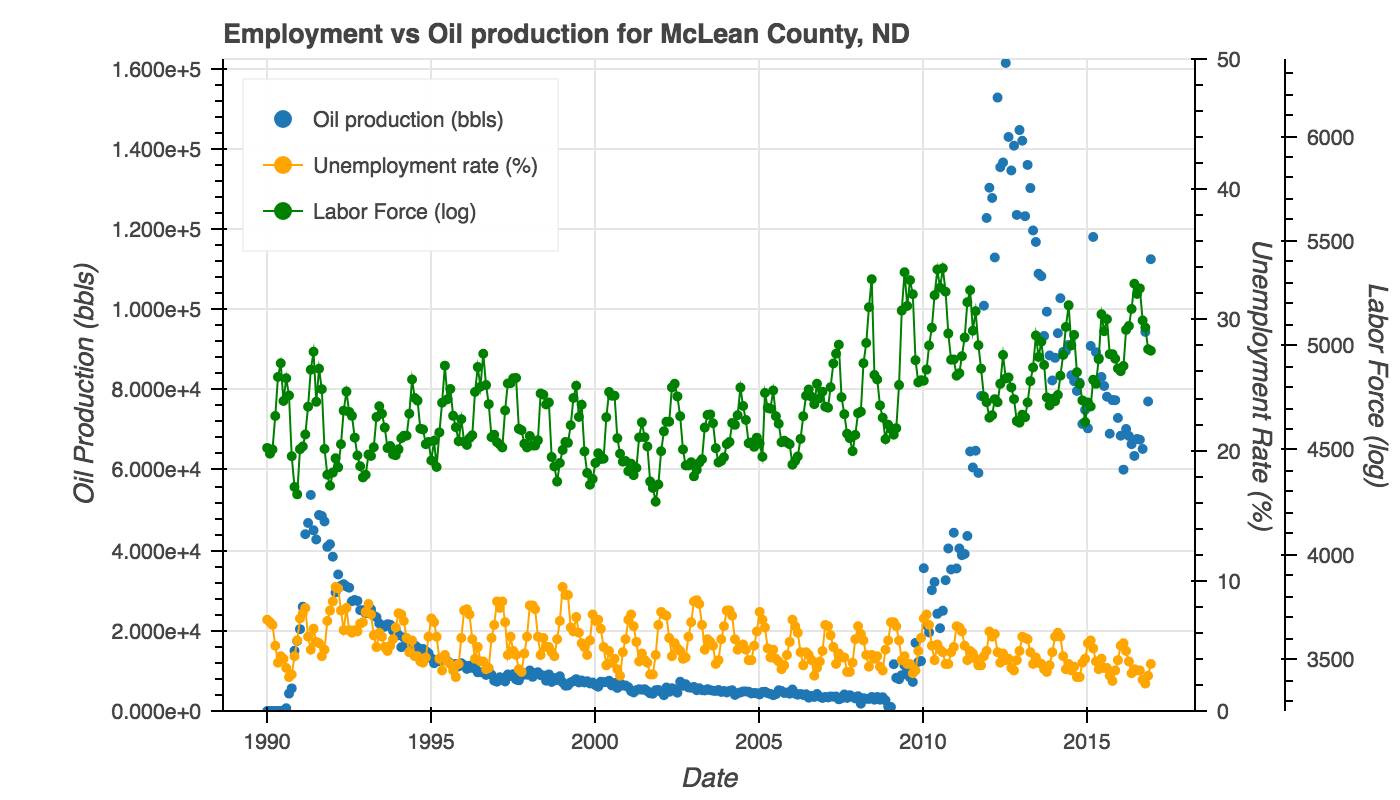
\includegraphics[width=1.1\linewidth]{nd_mclean_oil_prod}
\end{subfigure}

\begin{subfigure}{0.45\textwidth}
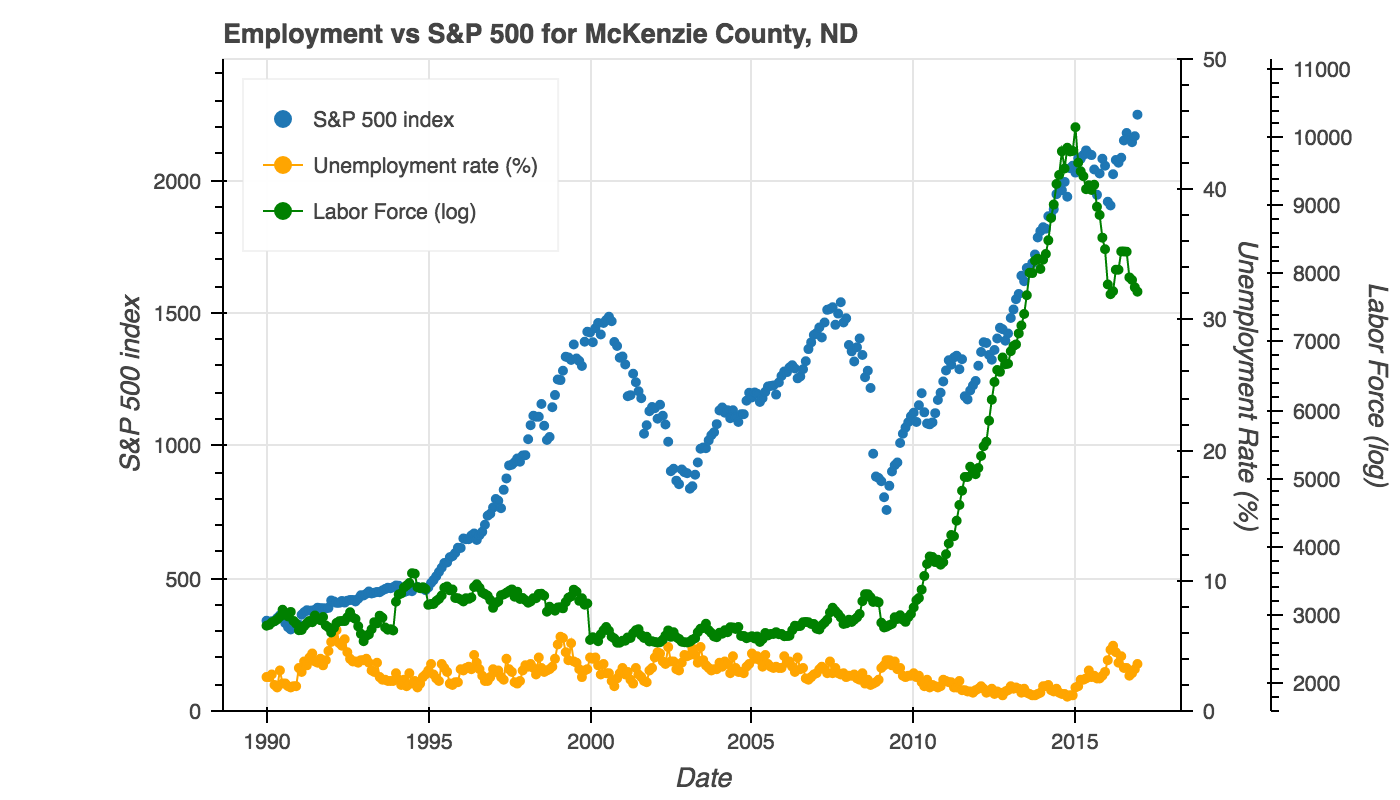
\includegraphics[width=1.1\linewidth]{nd_mckenzie_snp}
\end{subfigure}
~
\begin{subfigure}{0.45\textwidth}
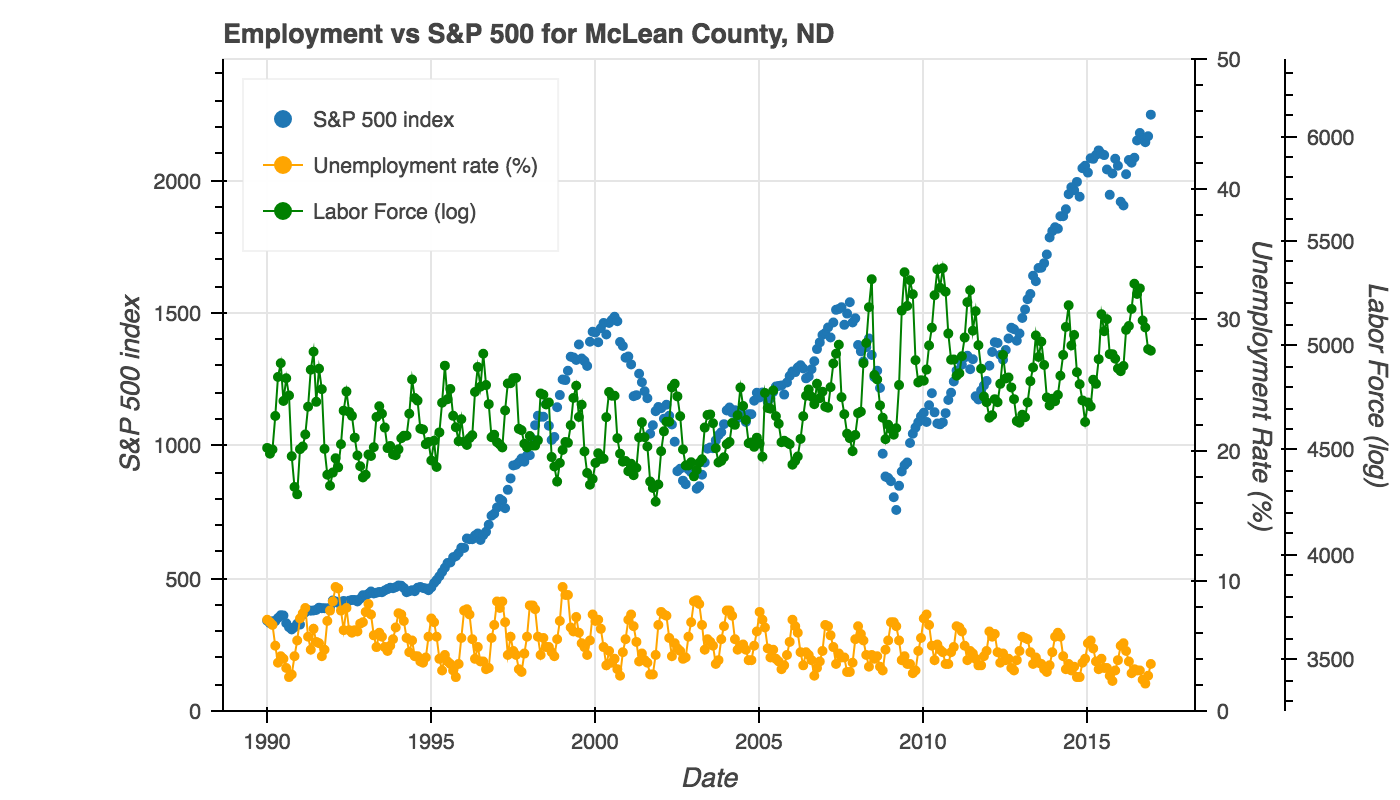
\includegraphics[width=1.1\linewidth]{nd_mclean_snp}
\end{subfigure}

\caption{The left column is for the high oil-producing McKenzie county, ND, while the right one is for the low-producing McLean county, ND. McKenzie county shows a dramatic increase in oil production in the 2000s, accompanied by a huge increase in the county labor force. While the unemployment rate in the county does show a sharp jump with the recent oil price crash in 2015, the much-increased labor force should also be taken into account here. Unlike McKenzie county, McLean county has significantly lower oil production, and does not seem to be affected much by the swings in oil prices.}
\label{fig:nd_hist_data}
\end{figure}


\subsection{Wyoming}

Figure \ref{fig:wy_maps} shows unemployment and oil production heat maps for Wyoming for three different years (1995, 2005, 2015). Similar to Texas and North Dakota, we see a trend towards decreasing levels of unemployment, although the heat map for production remains the same. 

Similar to Texas and North Dakota, we pick two counties with sharply contrasting levels of oil production, to see the effect of oil price on unemployment in these counties. Figure \ref{fig:wy_hist_data} shows data from Sublette county (a high oil producer) and Sheridan county (a low oil producer). As before, oil price swings have little to no impact on unemployment in Sheridan county. The main fluctuation in the unemployment rate for Sheridan county corresponds to the 2008 recession, which is captured in the sharp drop in the S\&P 500 index.

\begin{figure}[h!]
\centering
\begin{subfigure}{0.3\textwidth}
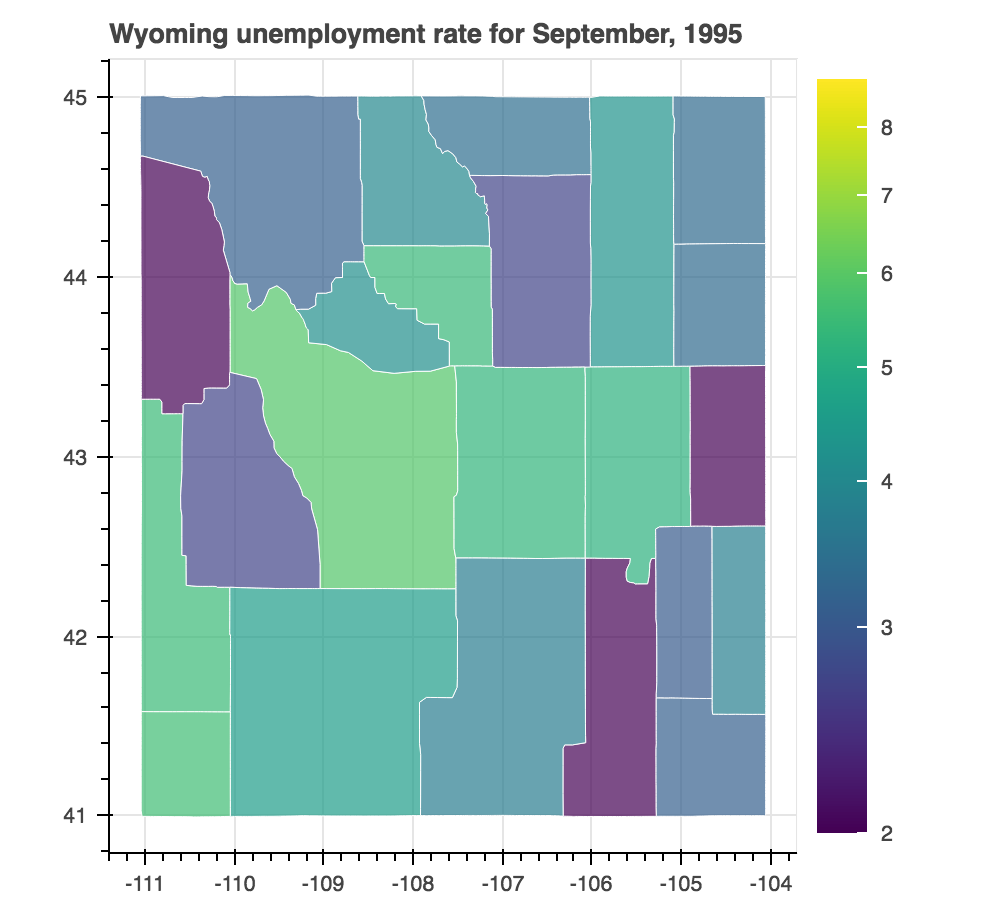
\includegraphics[width=1.2\linewidth]{wy_unemp_1995}
\end{subfigure}
~
\begin{subfigure}{0.3\textwidth}
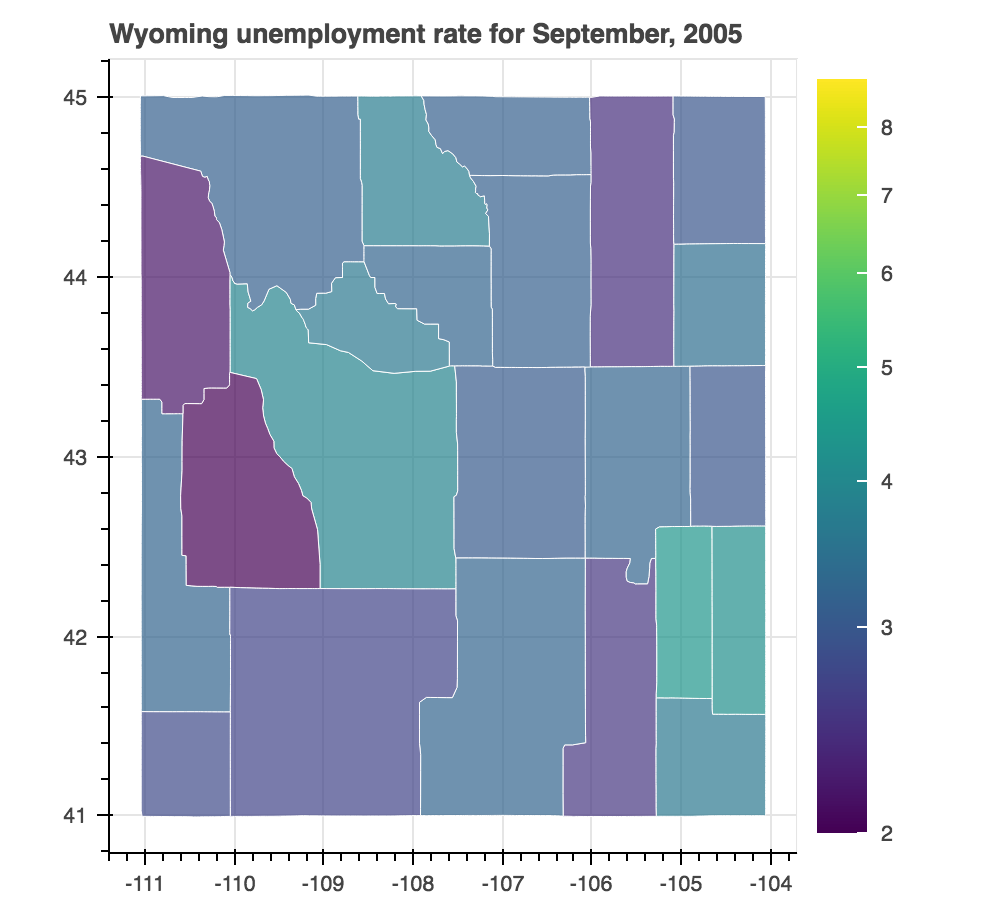
\includegraphics[width=1.2\linewidth]{wy_unemp_2005}
\end{subfigure}
~
\begin{subfigure}{0.3\textwidth}
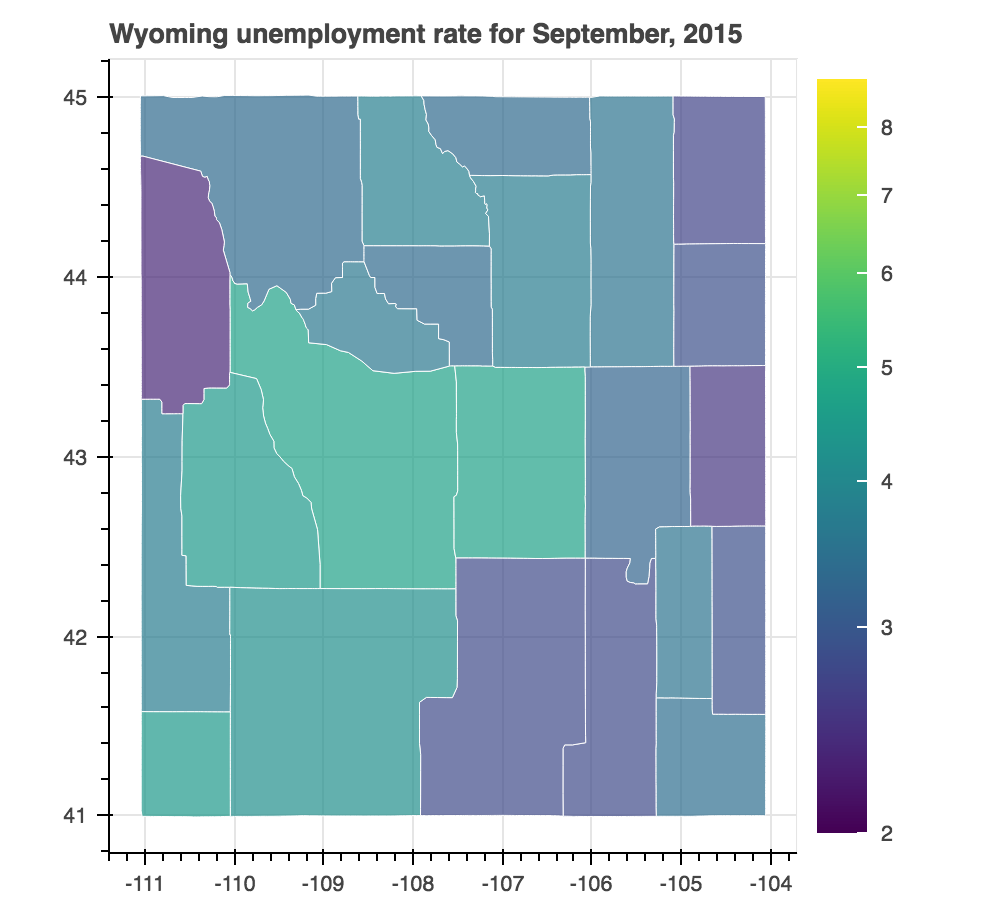
\includegraphics[width=1.2\linewidth]{wy_unemp_2015}
\end{subfigure}

\begin{subfigure}{0.3\textwidth}
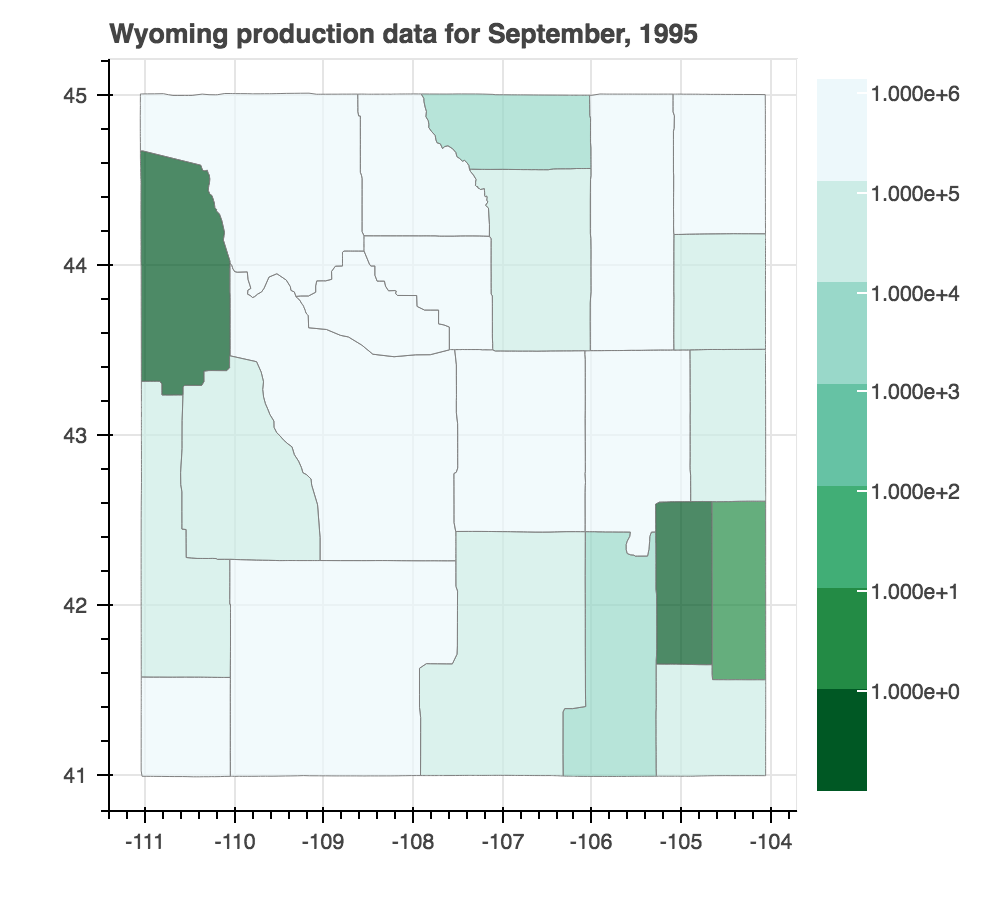
\includegraphics[width=1.2\linewidth]{wy_prod_1995}
\end{subfigure}
~
\begin{subfigure}{0.3\textwidth}
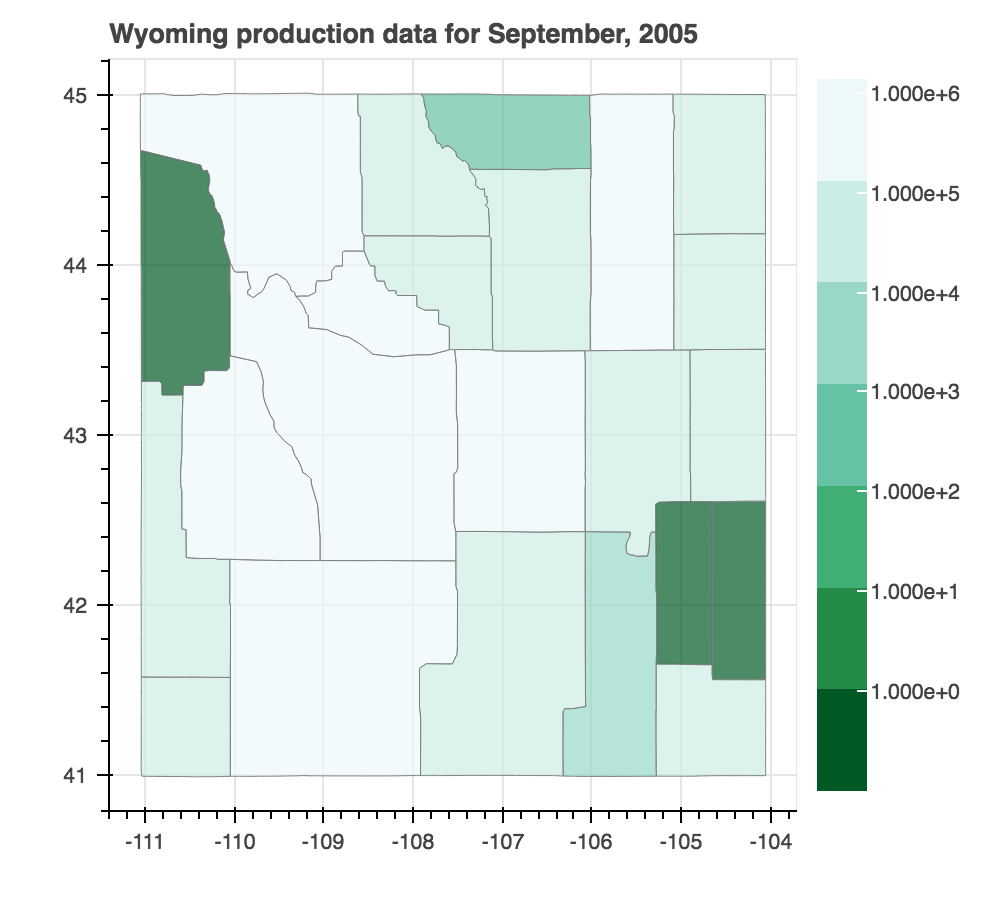
\includegraphics[width=1.2\linewidth]{wy_prod_2005}
\end{subfigure}
~
\begin{subfigure}{0.3\textwidth}
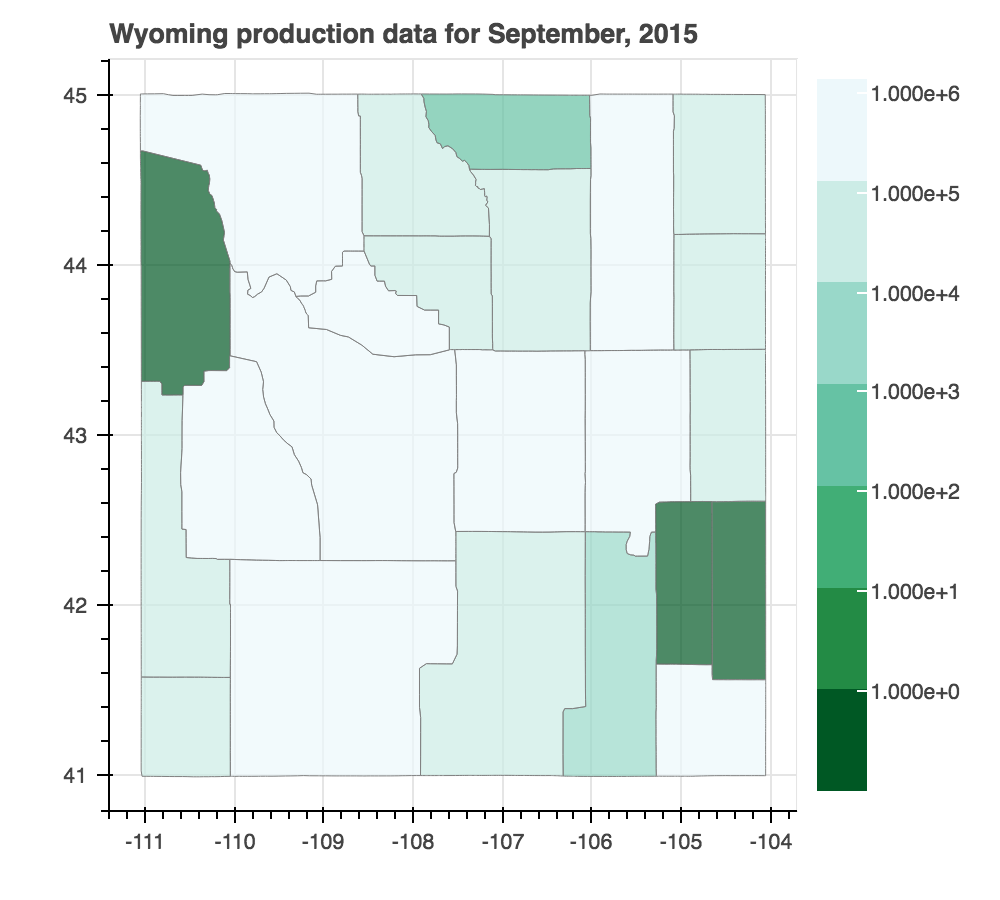
\includegraphics[width=1.2\linewidth]{wy_prod_2015}
\end{subfigure}
\caption{Wyoming trends: The top row shows evolution of unemployment rates in Wyoming from 1995-2015, while the bottom row shows oil production data. Same as the other states, the maps show decreasing unemployment overall in the state, specifically in the oil-producing counties.}
\label{fig:wy_maps}
\end{figure}

\begin{figure}
\centering
\begin{subfigure}{0.45\textwidth}
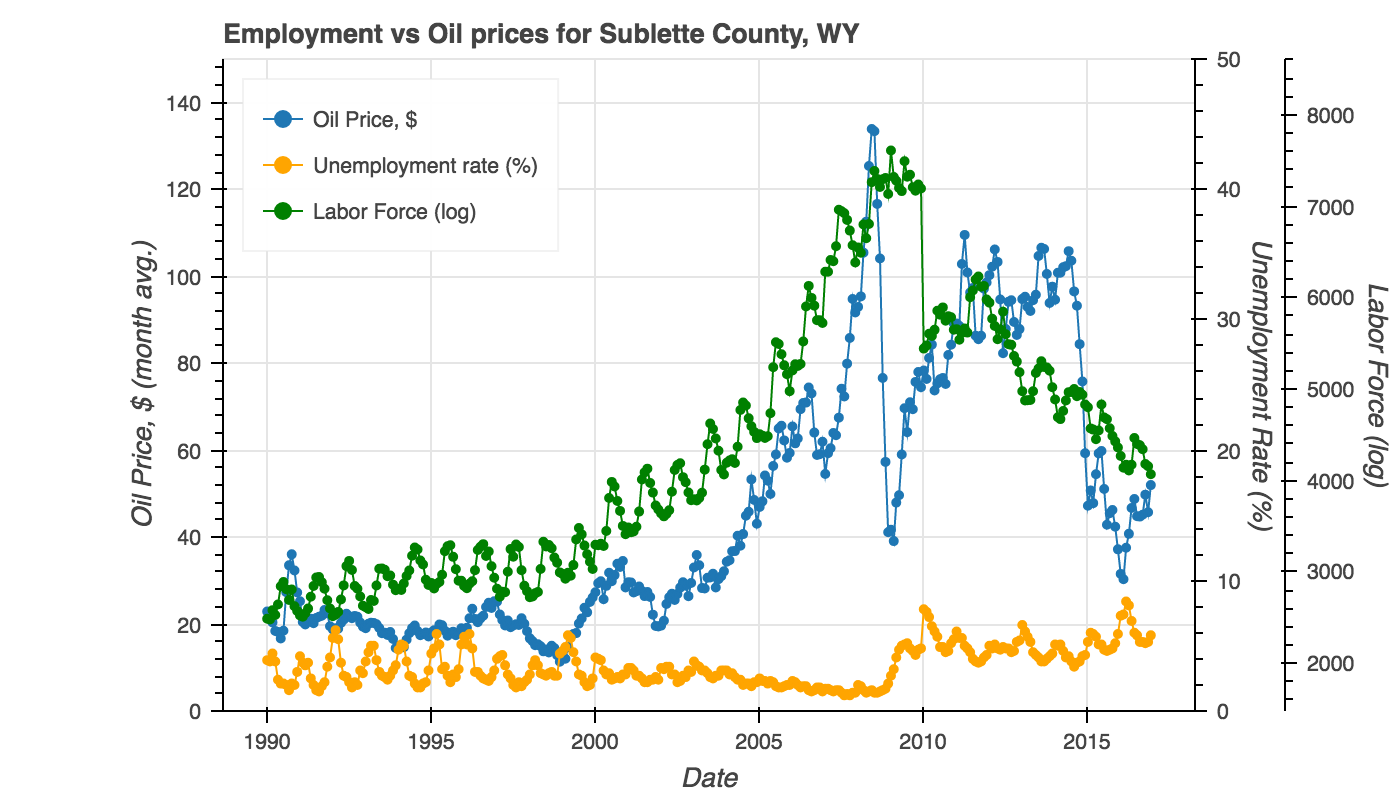
\includegraphics[width=1.1\linewidth]{wy_sublette_oil_price}
\end{subfigure}
~
\begin{subfigure}{0.45\textwidth}
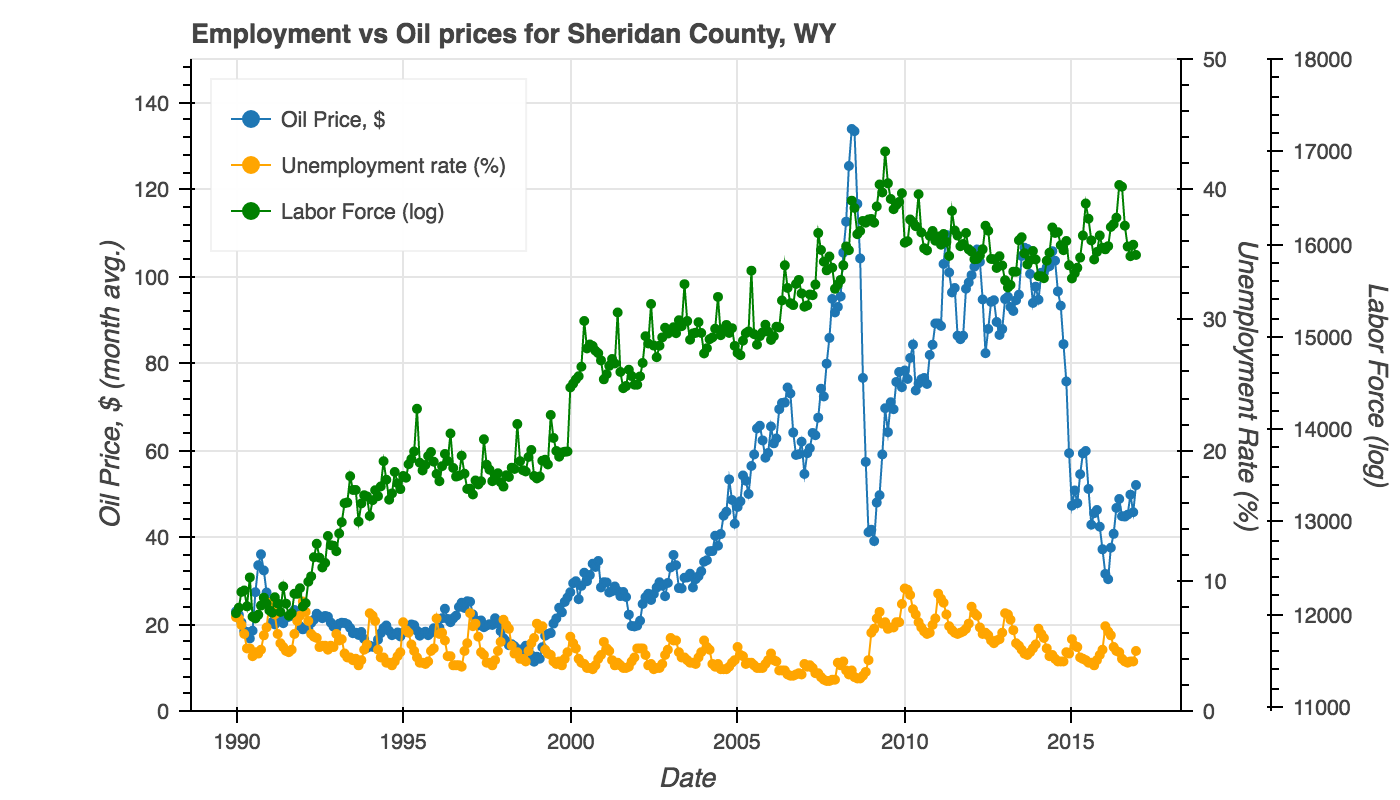
\includegraphics[width=1.1\linewidth]{wy_sheridan_oil_price}
\end{subfigure}

\begin{subfigure}{0.45\textwidth}
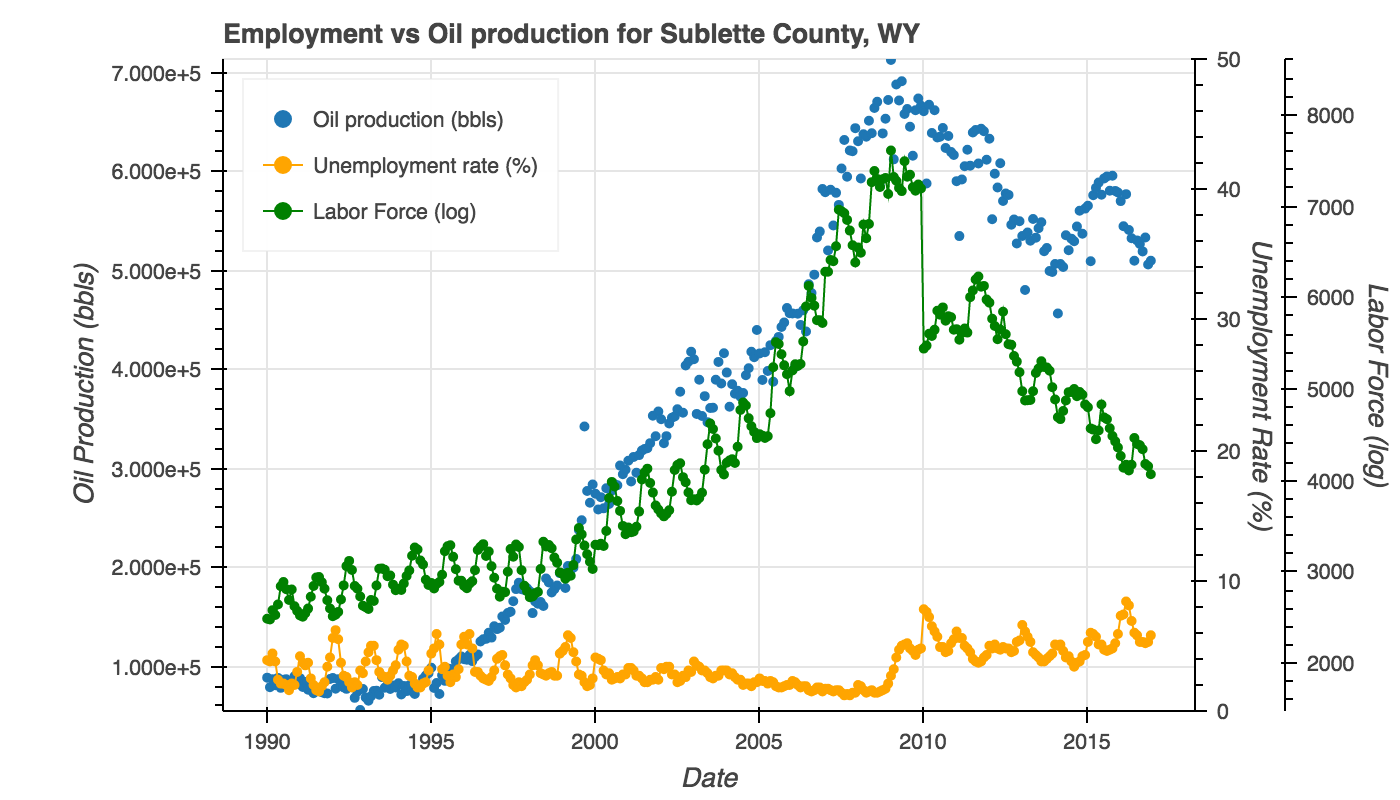
\includegraphics[width=1.1\linewidth]{wy_sublette_oil_prod}
\end{subfigure}
~
\begin{subfigure}{0.45\textwidth}
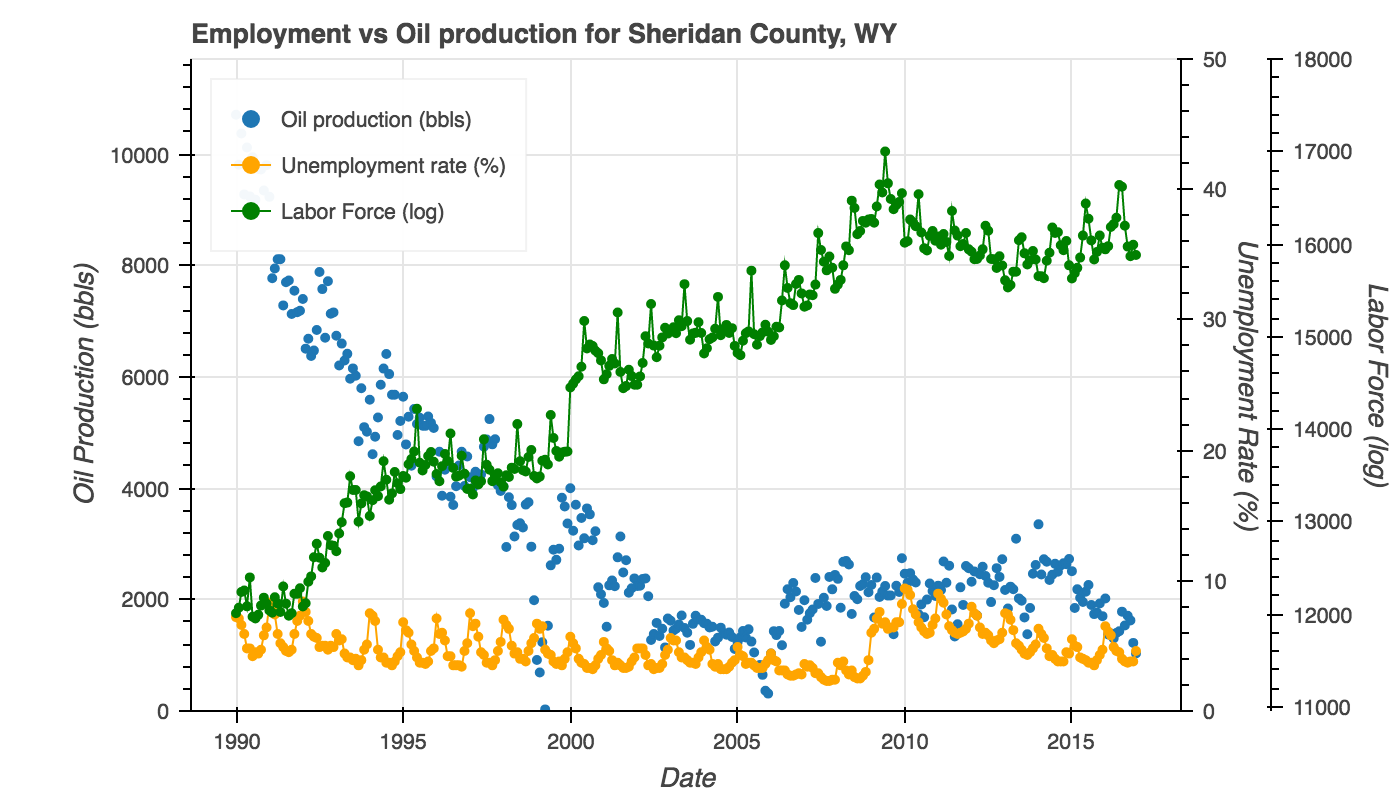
\includegraphics[width=1.1\linewidth]{wy_sheridan_oil_prod}
\end{subfigure}

\begin{subfigure}{0.45\textwidth}
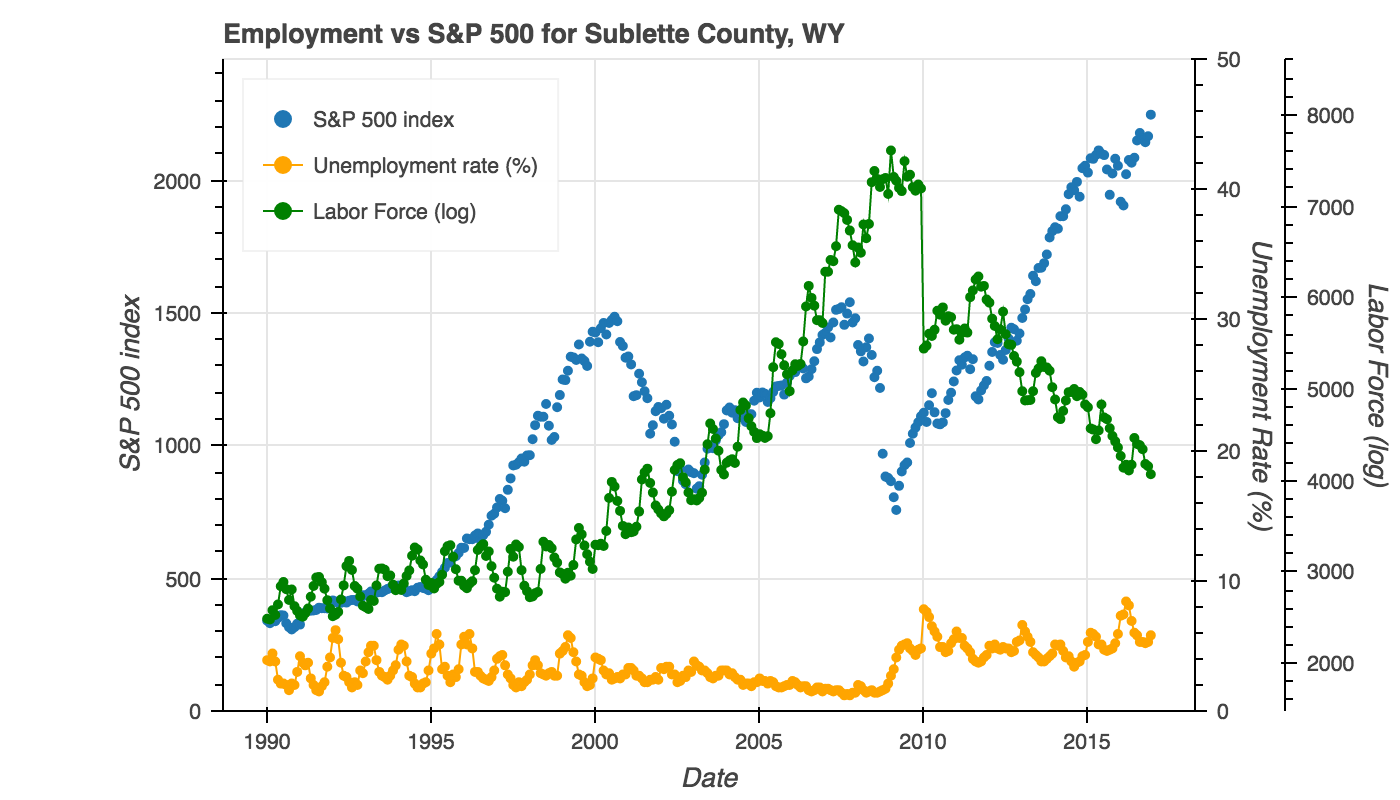
\includegraphics[width=1.1\linewidth]{wy_sublette_snp}
\end{subfigure}
~
\begin{subfigure}{0.45\textwidth}
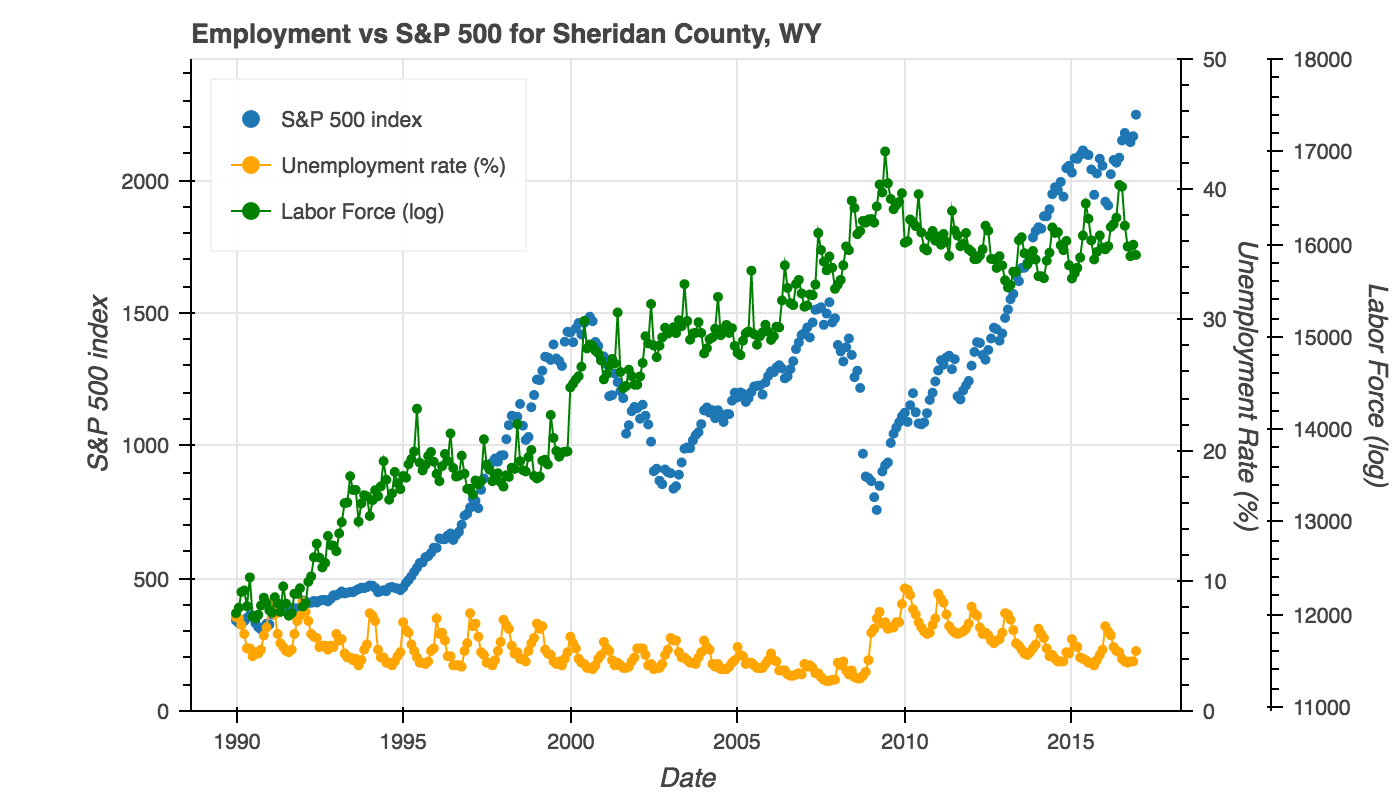
\includegraphics[width=1.1\linewidth]{wy_sheridan_snp}
\end{subfigure}

\caption{The left column shows data for Sublette county, WY, a high oil-producing region in Wyoming which displays strong dependence on oil prices. The right column shows Sheridan county, WY - a low oil-producing region in Wyoming, this county has maintained steady levels of unemployment throughout, except during times of wider economic recessions (such as in 2008).}
\label{fig:wy_hist_data}
\end{figure}

\section{Inferential Statistics}

In this section, I find the most important features for each county using Random Forest regression. Note that for this task one must use the 'RandomForestRegressor' instead of 'RandomForestClassifier' as we are dealing with continuous data. For each county, the historical unemployment rates, labor force and oil production data are extracted, and the oil price and S\&P 500 index data is added to it. Then a random forest is fit to the data.

The random forest package in scikit-learn produces a feature importance number, using which one can find out the most important feature. Using this, one can find the most important feature for determining unemployment rate for each county. 

I executed this step for all counties, for each 3 states. Figure \ref{fig:feature_maps} shows the results. It shows that the determining feature for unemployment rate is not necessarily oil production and/or oil price, even in counties with high oil production. As such, it is a multi-variate problem, and multiple factors must be taken into account.

\begin{figure}[h!]
\centering
\begin{subfigure}{0.4\textwidth}
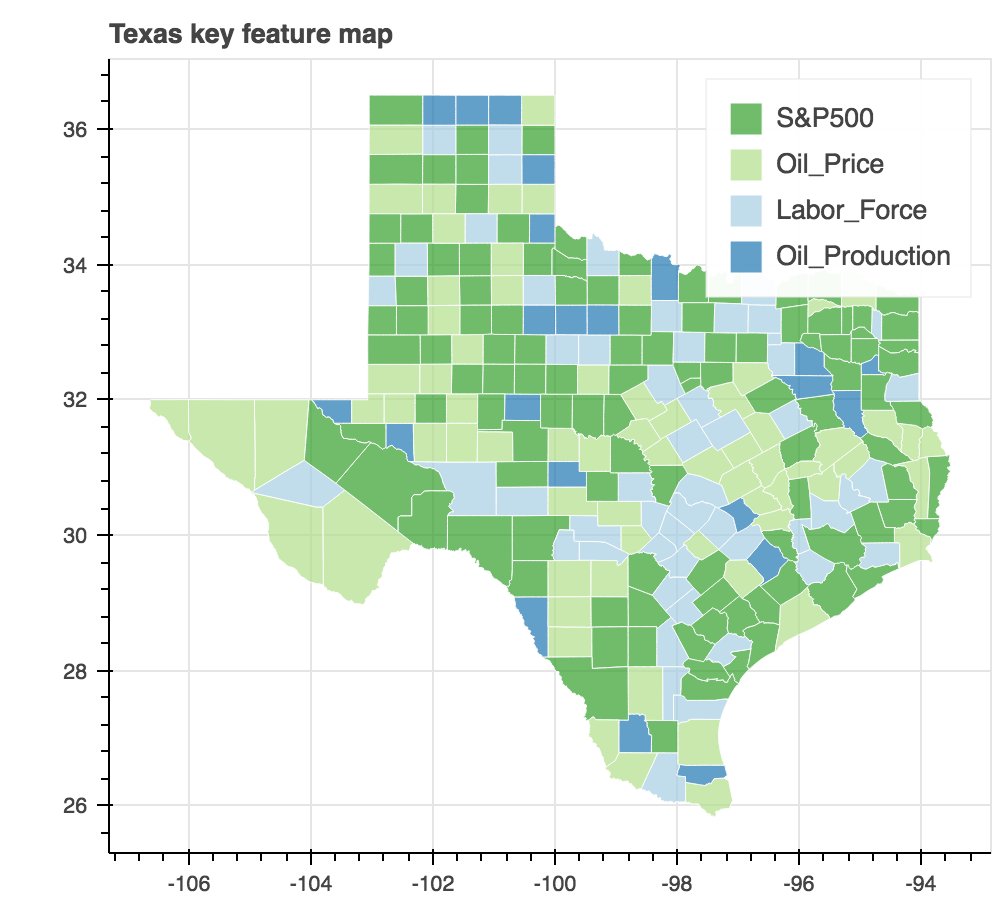
\includegraphics[width=\linewidth]{tx_feature}
\end{subfigure}
~
\begin{subfigure}{0.4\textwidth}
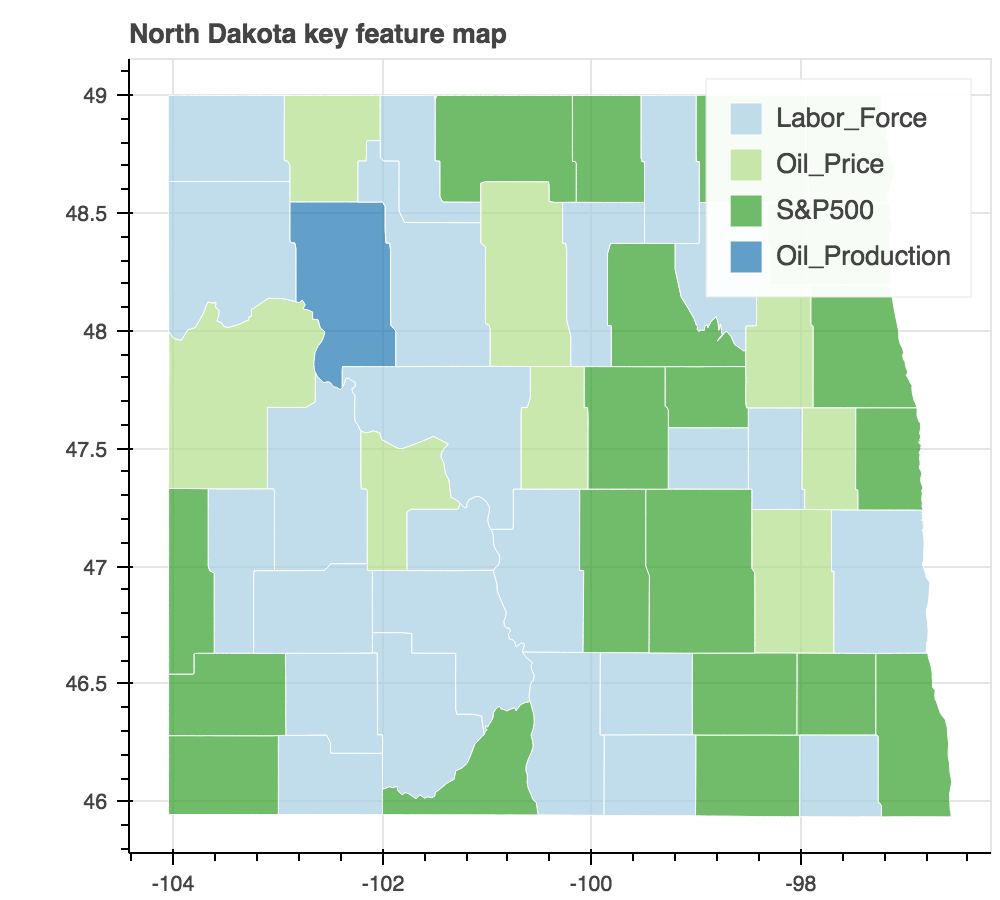
\includegraphics[width=\linewidth]{nd_feature}
\end{subfigure}

\begin{subfigure}{0.4\textwidth}
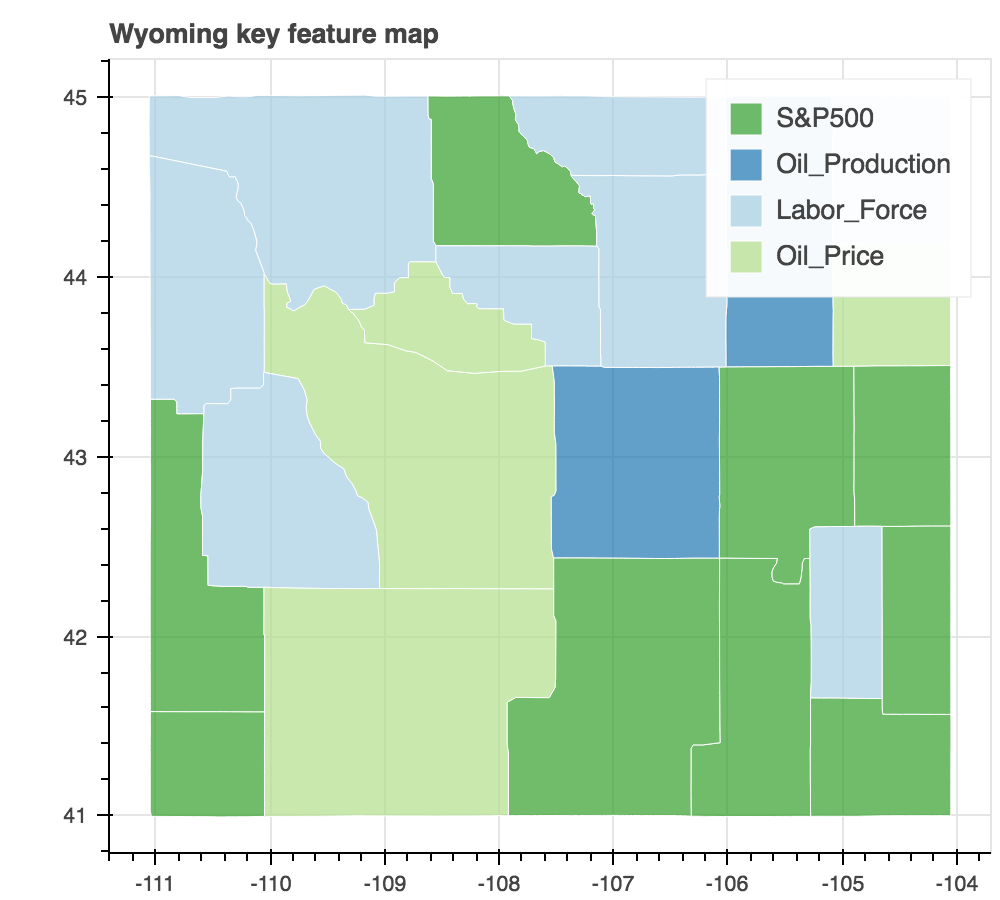
\includegraphics[width=\linewidth]{wy_feature}
\end{subfigure}
\caption{Feature maps for all three states, showing the most important feature for each county.}
\label{fig:feature_maps}
\end{figure}

\section{Conclusion}
The inferential statistics show that even for high oil-producing counties, national-level factors such as the S\&P 500 are more important in determining local area unemployment rates. This is not altogether surprising - for some of these counties, oil revenues have been high for such a long time that the economy has diversified, and a large complex economy should not be dependent on just the fortunes of one industry. 

This is also in contrast to the Enigma Labs project, which concludes that oil production is producing diminishing returns for North Dakota. My analysis indicates the situation is more complex - oil producing counties have experienced swings in employment levels for the past several decades. In counties where the oil boom has been for only a short period of time, this has led to over-dependence on the oil industry. However, counties with a longer history of oil production can rely on other industries during downturns in oil prices.

One question posed at the starting of this project was what would happen to the economies of counties dependent on the oil industry if the US transitions to a carbon-free economy. This project is nowhere ambitious enough to answer that question definitively - but from the data analysis, one can conclude that these counties should put in all of the surplus oil revenues into diversifying their economy, so that if and when another oil price crash happens, or oil is no longer needed anymore, they are still fine. Having said that, even with electric cars becoming increasingly common on the roads, it is unlikely oil and gas will be completely replaced anytime soon.

\end{document}
